\documentclass{beamer}
\mode<presentation>
\usepackage{algorithm,amssymb,amsmath,amsthm,bbm,color,epstopdf,float,geometry,graphicx,hyperref,listings,mathrsfs,mathtools,multirow,subcaption,textgreek,xcolor}
\usepackage[noend]{algpseudocode}
\usepackage[flushleft]{threeparttable}
\usepackage[shortlabels]{enumitem}

% Create Background Pic
%\usepackage{tikz}
%\definecolor{bottomcolour}{rgb}{0.32,0.3,0.38}
%\definecolor{topcolour}{rgb}{0.08,0.08,0.16}
%\setbeamertemplate{background canvas}{%
%	\begin{tikzpicture}[remember picture,overlay]
%	\shade[top color=topcolour,bottom color=bottomcolour]
%(current page.north west) rectangle (current page.south east);
%	\end{tikzpicture}%     
%}


%=======================================================
% Set page number
\setbeamertemplate{footline}[page number]

%=======================================================
%\usetheme{Boadilla}
\setbeamerfont{title}{size=\fontsize{18pt}{18pt}\selectfont} % bold font: \bfseries
\setbeamerfont{author}{size=\fontsize{20pt}{20pt}\selectfont}
\setbeamerfont{institute}{size=\fontsize{13pt}{13pt}\selectfont}
%\setbeamercolor{itemize item}{fg=red}

%================================================
%Set font color
\definecolor{mygray1}{rgb}{0.7421875,0.7421875,0.7421875}
\definecolor{mygray2}{gray}{0.6}
\definecolor{mygray3}{rgb}{0.55, 0.52, 0.54}
\definecolor{mybrown1}{rgb}{0.28, 0.24, 0.2}
\definecolor{myred}{rgb}{0.68, 0.09, 0.13}
\definecolor{myginger}{rgb}{0.69, 0.4, 0.0}
\definecolor{myblue1}{rgb}{0.0, 0.2, 0.6}
\definecolor{myblue2}{rgb}{0.38, 0.51, 0.71}
\definecolor{myblue3}{rgb}{0.2,0.2,0.7}
\definecolor{mygreen}{rgb}{0.42, 0.56, 0.14}
\definecolor{myviolet}{rgb}{0.54, 0.17, 0.89}


\newcommand{\highlightA}[1]{\colorbox{myblue3!50!}{$\displaystyle #1$}}
\newcommand{\highlightB}[1]{\colorbox{myred!50!}{$\displaystyle #1$}}
\newcommand{\highlightC}[1]{\colorbox{mygreen!50!}{$\displaystyle #1$}}
%================================================
% set picture source
\usepackage[absolute,overlay]{textpos}

\setbeamercolor{framesource}{fg=gray}
\setbeamerfont{framesource}{size=\tiny}
\newcommand{\source}[1]{\begin{textblock*}{4cm}(8.7cm,8.6cm)
\begin{beamercolorbox}[ht=0.5cm,right]{framesource}
\usebeamerfont{framesource}\usebeamercolor[fg]{framesource} Source: {#1}
\end{beamercolorbox}
\end{textblock*}}

\setbeamercolor{frametitle}{fg=white,bg=black}


%================================================
% url color
\renewcommand\UrlFont{\color{myblue3}}
%================================================

\newtheorem{Thm}{{\bf Theorem}}


% Make first page
\makeatletter
\setbeamertemplate{navigation symbols}{}
\title[Grad-Shafranov]{\Large  
Efficient Computational Algorithms for the Grad-Shafranov Free Boundary Problem}
%\subtitle[short version]{}
%\date{}
\author[Jiaxing Liang]{\normalsize Jiaxing Liang (Rice Univeristy),\\
\vspace{4mm}
Howard Elman (UMD, College Park),\\
Tonatiuh S\'anchez-Vizuet (University of Arizona),\\
Matthias Heinkenschloss (Rice Univeristy).}
\vspace{-5cm}
%\institute[UMD]{University of Maryland, College Park}
%\usetheme{Pittsburgh}
%\usecolortheme{owl}

%======Footline=================================================
%\makeatother
%\setbeamertemplate{footline}
%{
%	\leavevmode%
%	\hbox{%
%%		\begin{beamercolorbox}[wd=.4\paperwidth,ht=2.25ex,dp=1ex,center]{author in head/foot}%
%%			\usebeamerfont{author in head/foot}\insertshortauthor
%%		\end{beamercolorbox}%
%		\begin{beamercolorbox}[wd=\paperwidth,ht=2.25ex,dp=1ex,leftskip=4.3cm,rightskip=.3cm plus1fil]{topcolour}
%			\usebeamerfont{title in head/foot}\insertshorttitle\hfill%\hspace*{3em}
%			\insertframenumber{} / \inserttotalframenumber\hspace*{1ex}
%	\end{beamercolorbox}}%
%\begin{beamercolorbox}[wd=.1\paperwidth,ht=2.25ex,dp=1ex,right,rightskip=2ex]{page number in head/foot}%
%	%            \usebeamerfont{title in head/foot}\insertshorttitle\hspace*{3em}
%	\insertframenumber{} / \inserttotalframenumber
%\end{beamercolorbox}%    
%	\vskip0pt%
%}

%=======================================================
\begin{document}
\frame{\titlepage }

%------------------------------------------------------------
\begin{frame}[c]		
\frametitle{Outline}
\normalsize
\begin{itemize}[leftmargin=5pt] 
\item[$\triangleright$] Physical Model: Grad-Shafranov Equation
\vspace{0.3cm}
\item[$\triangleright$] Uncertainty Quantification 
\vspace{0.3cm}
\item[$\triangleright$] Objectives
% \vspace{0.3cm}
% \item[$\triangleright$] Surrogate via Sparse Grid Stochastic Collocation
\vspace{0.3cm}
\item[$\triangleright$] Approach 1: Surrogate-based Monte Carlo
    % \vspace{0.3cm}
    % {\footnotesize
    % \begin{itemize}[leftmargin=15pt]   
    %     \item[$\circ$] \textcolor{mygray3}{Surrogate via Sparse Grid Stochastic Collocation}
    %     % \vspace{0.3cm}
    %     \item[$\circ$] \textcolor{mygray3}{Experimental Results \& Conclusions}
    % \end{itemize}
    % }
\item[$\triangleright$] Approach 2: Multilevel Monte Carlo with Non-linear Solve
    % \vspace{0.3cm}
    % {\footnotesize
    % \begin{itemize}[leftmargin=15pt]   
    %     \item[$\circ$] \textcolor{mygray3}{Monte Carlo \& Uniform Multilevel Monte Carlo}
    %     \item[$\circ$] \textcolor{mygray3}{Adaptive Multilevel Monte Carlo}
    %     \item[$\circ$] \textcolor{mygray3}{Experimental Results \& Conclusions}
    % \end{itemize}
    % }
\item[$\triangleright$] Approach 3: Surrogate-based Multilevel Monte Carlo
    % {\footnotesize
    % \begin{itemize}[leftmargin=15pt]   
    %     \item[$\circ$] \textcolor{mygray3}{Three Types of Surrogates}
    %     \item[$\circ$] \textcolor{mygray3}{Surrogate-based Samplings}
    %     \item[$\circ$] \textcolor{mygray3}{Experimental Results \& Conclusions}
    % \end{itemize}
    % }
\item[$\triangleright$] Approach 4: Multi-fidelity Monte Carlo
\end{itemize}
\end{frame}


%------------------------------------------------------------
\begin{frame}[c]
\setbeamercolor{itemize item}{fg=mygray1}
\large 	
\textcolor{mygray1}{
    \begin{itemize}[leftmargin=5pt] 
        \item[\textcolor{black}{$\triangleright$}] \textcolor{black}{\fontsize{25}{60}\selectfont Physical Model: Grad-Shafranov Equation}
        \vspace{0.2cm}	
        \item[$\triangleright$] Uncertainty Quantification
        \vspace{0.2cm}
        \item[$\triangleright$] Objectives
        \vspace{0.2cm}
        \item[$\triangleright$] Approach 1: Surrogate-based Monte Carlo
            % \vspace{0.3cm}
            % {\footnotesize
            % \begin{itemize}[leftmargin=15pt]   
            %     \item[$\circ$] Surrogate via Sparse Grid Stochastic Collocation
            %     % \vspace{0.3cm}
            %     \item[$\circ$] Experimental Results \& Conclusions
            % \end{itemize}
            % }
        \vspace{0.2cm}
        \item[$\triangleright$] Approach 2: Multilevel Monte Carlo with Non-linear Solve
            % \vspace{0.3cm}
            % {\footnotesize
            % \begin{itemize}[leftmargin=15pt]   
            %     \item[$\circ$] Monte Carlo \& Uniform Multilevel Monte Carlo
            %     \item[$\circ$] Adaptive Multilevel Monte Carlo
            %     \item[$\circ$] Experimental Results \& Conclusions
            % \end{itemize}
            % }
        \vspace{0.2cm}
        \item[$\triangleright$] Approach 3: Surrogate-based Multilevel Monte Carlo
            % {\footnotesize
            % \begin{itemize}[leftmargin=15pt]   
            %     \item[$\circ$] Three Types of Surrogates
            %     \item[$\circ$] Surrogate-based Samplings
            %     \item[$\circ$] Experimental Results \& Conclusions
            % \end{itemize}
            % }
        \vspace{0.2cm}
        \item[$\triangleright$] Approach 4: Multi-fidelity Monte Carlo
    \end{itemize}
}
\end{frame}
%------------------------------------------------------------



\begin{frame}[t]{stellar}
\frametitle{Fusion \& Magnetic Confinement}
{\footnotesize
\begin{itemize}[leftmargin=5pt] 
    \item[$\triangleright$]  \textcolor{myblue3}{\bf \normalsize Fusion reactor:} Focus on Tokamak -- doughnut-shaped vacuum chamber. 
    
    \item[$\triangleright$] \textcolor{myblue3}{\bf\normalsize  Fusion mechanism:} Inject fuel gas (hydrogen isotopes) into the chamber $\rightarrow$ heated with microwave $\rightarrow$ form a plasma $\rightarrow$ particles overcome coulomb repulsion $\rightarrow$ fuse to produce energy.
    
    \vspace{0.1cm}
    \begin{figure}[H]	
    \centering
    \begin{tabular}{ccc}
    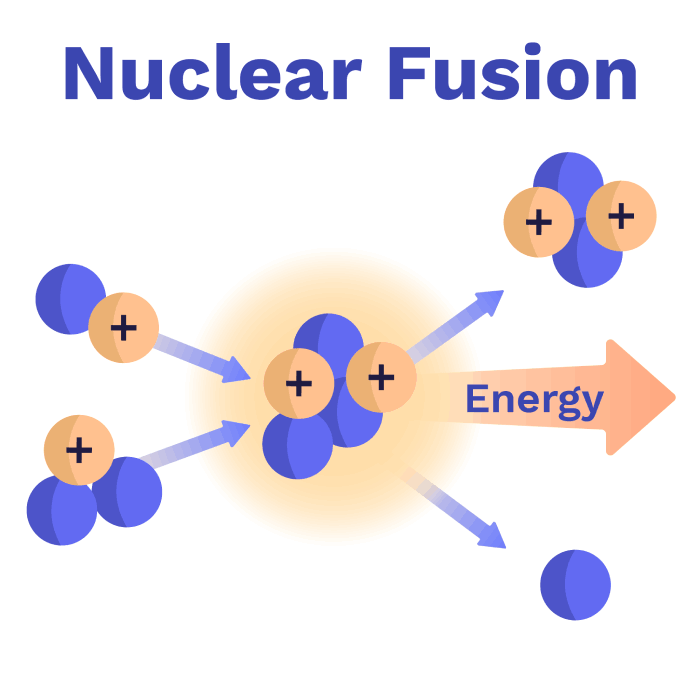
\includegraphics[height=0.2\linewidth]{fusion_reaction.png}&\qquad \qquad
    \includegraphics[height=0.2\linewidth]{ITER}&
    % \includegraphics[height=0.26\linewidth]{"IterChamber"}
    \end{tabular}
    \source{https://www.iter.org/mach/Tokamak}
    \end{figure}

        \item[$\triangleright$] During fusion, the hot plasma tends to expand, to prevent it from contacting the reactor wall, it must be confined. 
        \item[$\triangleright$] \textcolor{myblue3}{\bf\normalsize  Magnetic confinement:} Confinement is achieved through magnetic fields generated by currents running through external coils surrounding the reactor.
        \item[$\triangleright$] Our project focuses on studying the \textcolor{myred}{\bf impact of variations in current} on the physical properties of the confinement field. These \textcolor{myred}{\bf variations} may come from power supply, temperature fluctuations, and material impurities in the conduction wire.
\end{itemize}
}	
\end{frame}



%------------------------------------------------------------
\begin{frame}[t]
\frametitle{The Grad-Shafranov Free Boundary Problem}
\vspace{-4mm}
\begin{minipage}[t]{\linewidth}
    {\footnotesize
        \begin{subequations}
            \begin{equation*}
            -\nabla\,\cdot\,\left(\frac{1}{\mu x}\nabla\psi\right) = \left\{ \begin{array}{ll}
            x\frac{d}{d\psi} p(\psi) + \frac{1}{2\, \mu x} \frac{d}{d\psi}  g^2(\psi) & \text{ in } \underline{\Omega_p(\psi)} \\
            \boldsymbol{I_i}/S_i & \text{ in } \Omega_{C_i} \\
            0 & \text{ elsewhere } 
            \end{array}\right.
            \end{equation*}
            \begin{equation*}
            \psi(0,y) = 0 ; \qquad \qquad  \lim_{\|(x,y)\|\to\infty}\psi(x,y) = 0. 
            \end{equation*}
        \end{subequations}}

{\footnotesize
              \begin{itemize}[leftmargin=0pt] 
                    \item[]	\textcolor{myblue3}{$\psi$:} \textcolor{mybrown1}{poloidal flux.}
                    \; \textcolor{myblue3}{$\mu(\psi)$:} \textcolor{mybrown1}{magnetic permeability.} 
                    \; \textcolor{myblue3}{$p(\psi)$:} \textcolor{mybrown1}{hydrodynamic pressure}.
                    
                    \vspace{-1.5mm}
                    \item[]	\textcolor{myblue3}{$g(\psi)$:}  \textcolor{mybrown1}{toroidal field function.}
                    \;\textcolor{myblue3}{$\Omega_p(\psi)$:} \textcolor{mybrown1}{confinement region.}
                    \;\textcolor{myblue3}{$I_i$:} \textcolor{mybrown1}{current intensity.}

                    \vspace{-1.5mm}
                    \item[]	\textcolor{myblue3}{$S_i$:} \textcolor{mybrown1}{cross section area of the coils.}\quad \textcolor{myblue3}{$\Omega_{c_i}$:} \textcolor{mybrown1}{locations of coils.}
                \end{itemize}
    }
    
    \begin{columns}
        %	\hspace{-3mm}
        \begin{column}{0.66\linewidth}
            {\small
                % \begin{itemize}[leftmargin=5pt] 
                %     \item[]	\textcolor{myblue3}{$\psi$:} \textcolor{mybrown1}{poloidal flux function.}
                %     \vspace{-1.5mm}
                %     %			\vspace{-5mm}
                %     \item[]	\textcolor{myblue3}{$p(\psi)$:} \textcolor{mybrown1}{hydrodynamic pressure}.
                %     \vspace{-1.5mm}
                %     %		\vspace{-4mm}
                %     \item[]	\textcolor{myblue3}{$I_i$:} \textcolor{mybrown1}{current intensity in the coils.}
                %     \vspace{-1.5mm}
                %     \item[]	\textcolor{myblue3}{$\Omega_p(\psi)$:} \textcolor{mybrown1}{confinement region.}
                %     \vspace{-1.5mm}
                %     \item[]	\textcolor{myblue3}{$\mu(\psi)$:} \textcolor{mybrown1}{magnetic permeability.}
                %     \vspace{-1.5mm} 
                %     \item[]	\textcolor{myblue3}{$g(\psi)$:}  \textcolor{mybrown1}{toroidal field function.}
                %     \vspace{-1.5mm}
                %     \item[]	\textcolor{myblue3}{$S_i$:} \textcolor{mybrown1}{cross section area of the coils.}
                %     \vspace{-1.5mm}
                %     \item[]	\textcolor{myblue3}{$\Omega_{c_i}$:} \textcolor{mybrown1}{locations of coils.}
                % \end{itemize}
            \vspace{-3mm}
            \begin{itemize}[leftmargin=40pt] 
            % \item[$\circ$] Physical space: 2-d.
            % \item[$\circ$] {\bf Knowns:} $ p(\psi), g(\psi), I_i, \Omega_{c_i}$, and  $\mu$. {\bf Unknowns:} $\psi$ and $\Omega_p(\psi)$.

            \item[$\circ$] {\bf Non-linear} \underline{free boundary problem} with the source of uncertainty arises from the \textcolor{myred}{\bf current intensities}.

            \item[$\circ$] {\bf Knowns:} $ p(\psi), g(\psi), I_i, \Omega_{c_i}$, and  $\mu$. {\bf Unknowns:} $\psi$ and $\Omega_p(\psi)$.
            
            \item[$\circ$] \textcolor{myblue3}{\bf Software:} \textsc{Matlab} finite element package {\tt FEEQS.M} -- H. Heumann and his collaborators.

        %     {\fontsize{7.5}{7.5}\selectfont \textcolor{mygray2}{
        % H. Heumann, J. Blum, C. Boulbe, B. Faugeras, G. Selig, J.-M. Ané, S. Brémond, V. Grandgirard, P. Hertout, E. Nardon, et al., Quasi-static free-boundary
        %     equilibrium of toroidal plasma with CEDRES: computational methods and applications, J. Plasma Phys. 81 (3) (2015) 905810301.}\par}
            \end{itemize}
            }
        \end{column}
        
        % \hspace{-3mm}
        \begin{column}{0.5\linewidth}
        \vspace{-6mm}
            \begin{figure}[H]	
                \centering
                \hspace{-17mm}
                \begin{tabular}{cc}
                    \begin{subfigure}{0.5\textwidth}
                    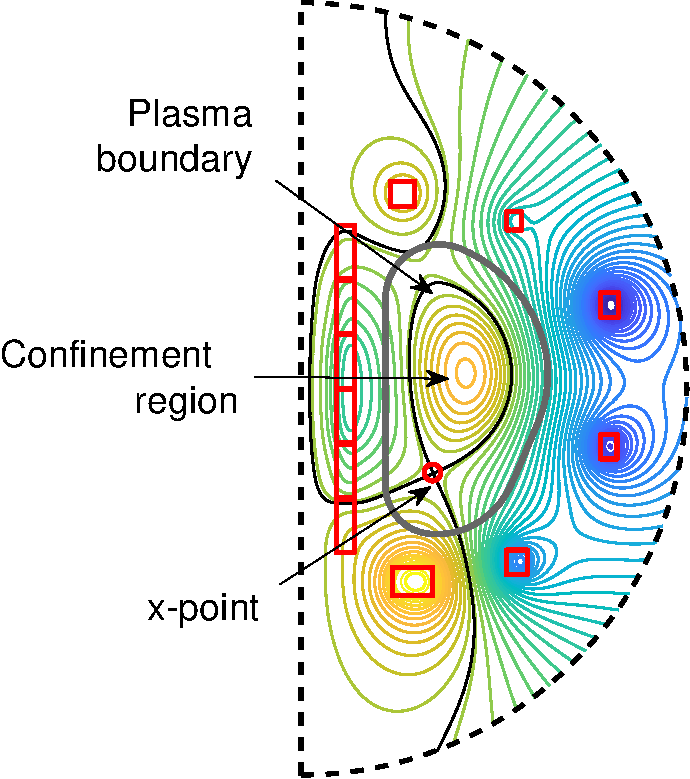
\includegraphics[height=1.8\linewidth]{FreeBoundary_contoursWstructures}
                        %					\caption*{Diverted configuration}
                    \end{subfigure}
                \end{tabular}
            \end{figure}
        \end{column}
    \end{columns}
\end{minipage}
\end{frame}

%------------------------------------------------------------
\begin{frame}[t]
\frametitle{Scenarios of Plasma Confinement}
    
\vspace{-2mm}

\begin{figure}[H]	
    \centering
    \hspace{10mm}
    \begin{tabular}{cc}
        \begin{subfigure}{0.4\textwidth}
            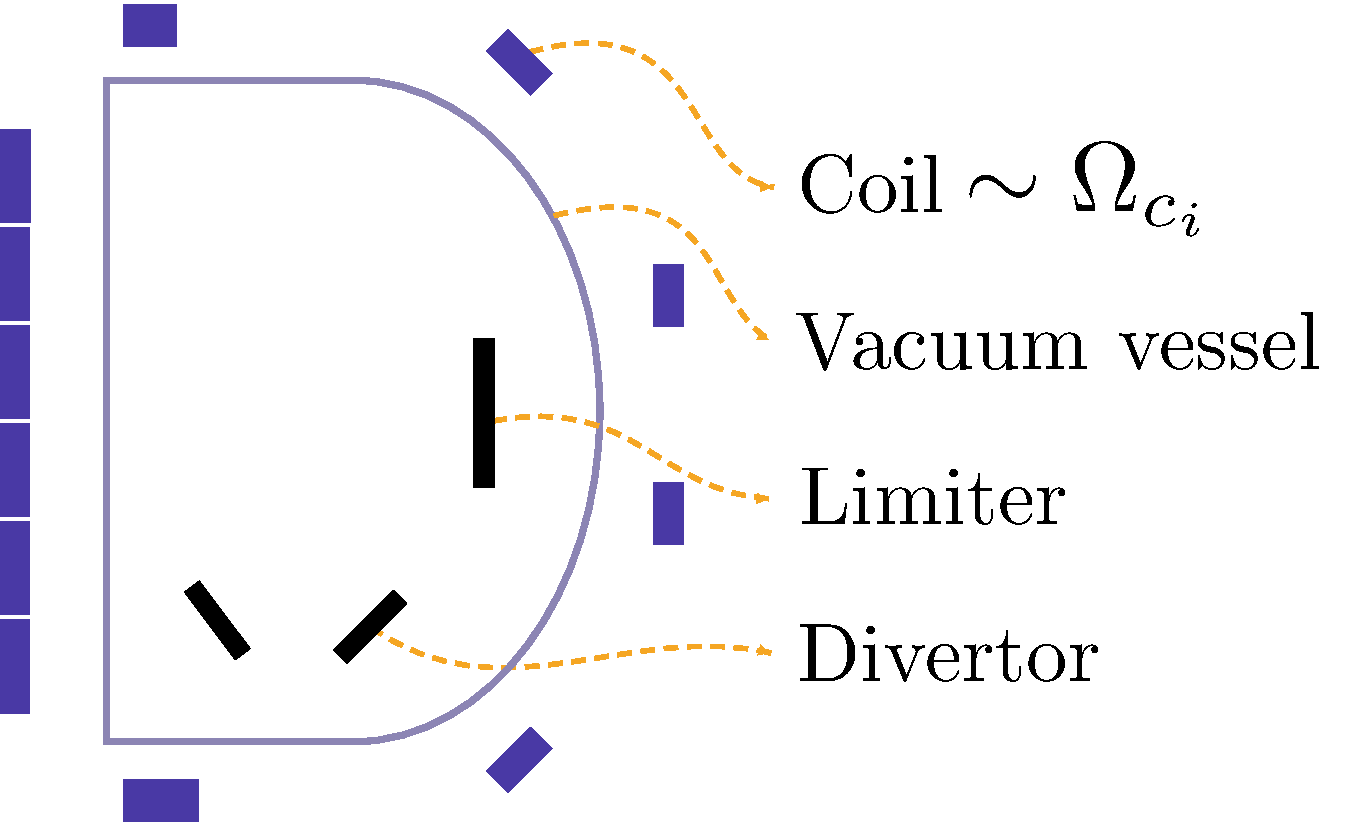
\includegraphics[height=0.45\linewidth]{BasicConfig}
            %					\caption*{Limited configuration}
        \end{subfigure}
        &
        % \hspace{-10mm}
        \begin{subfigure}{0.4\textwidth}
            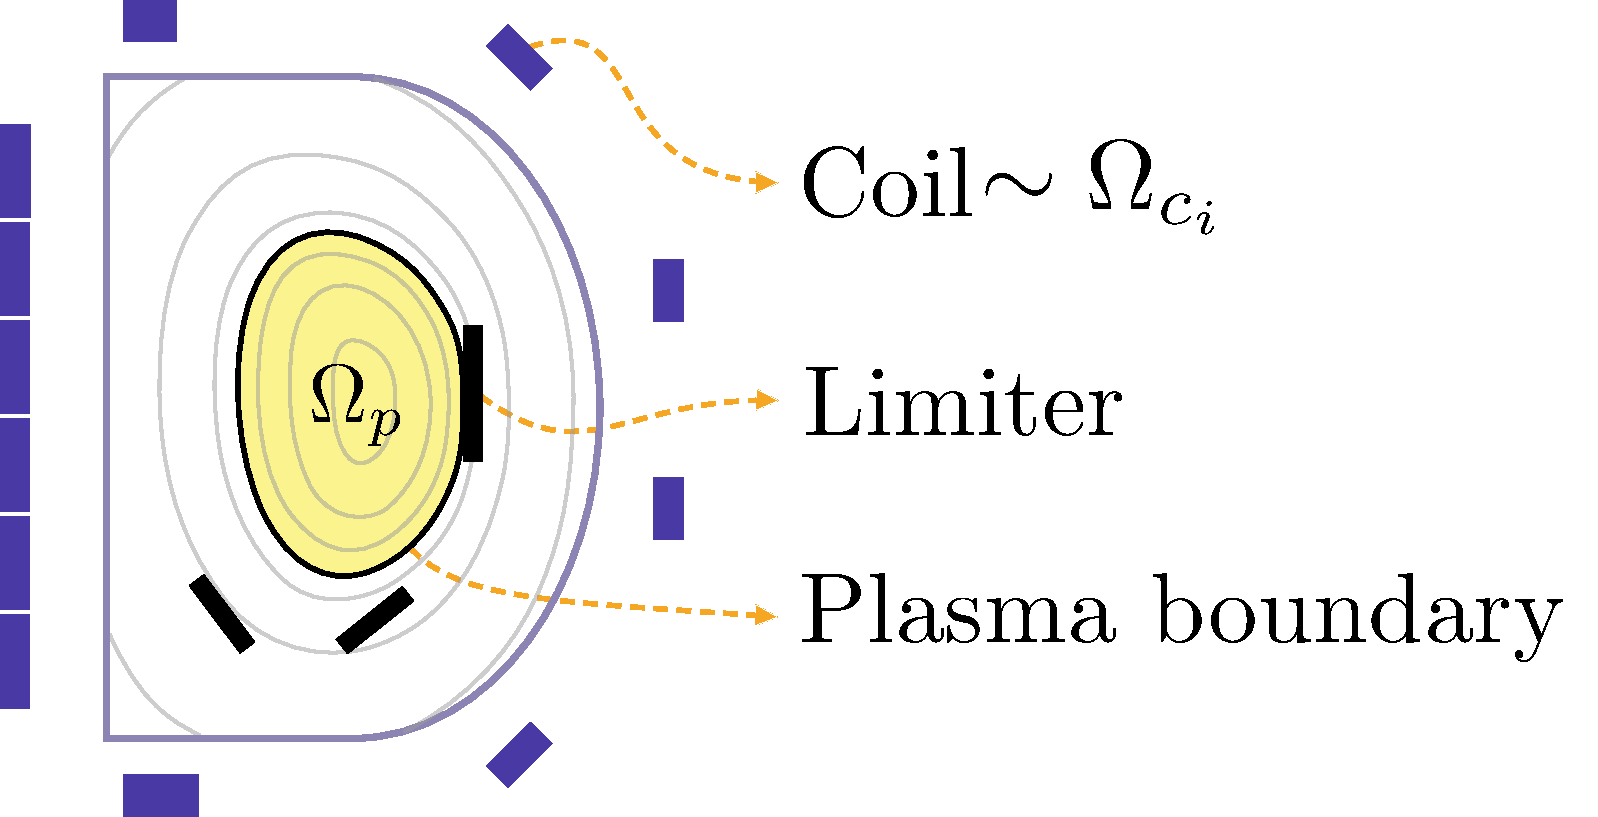
\includegraphics[height=0.45\linewidth]{Limiter}
            %					\caption*{Diverted configuration}
        \end{subfigure}\\
        Empty & Limited\\ [1ex]
        \begin{subfigure}{0.4\textwidth}
            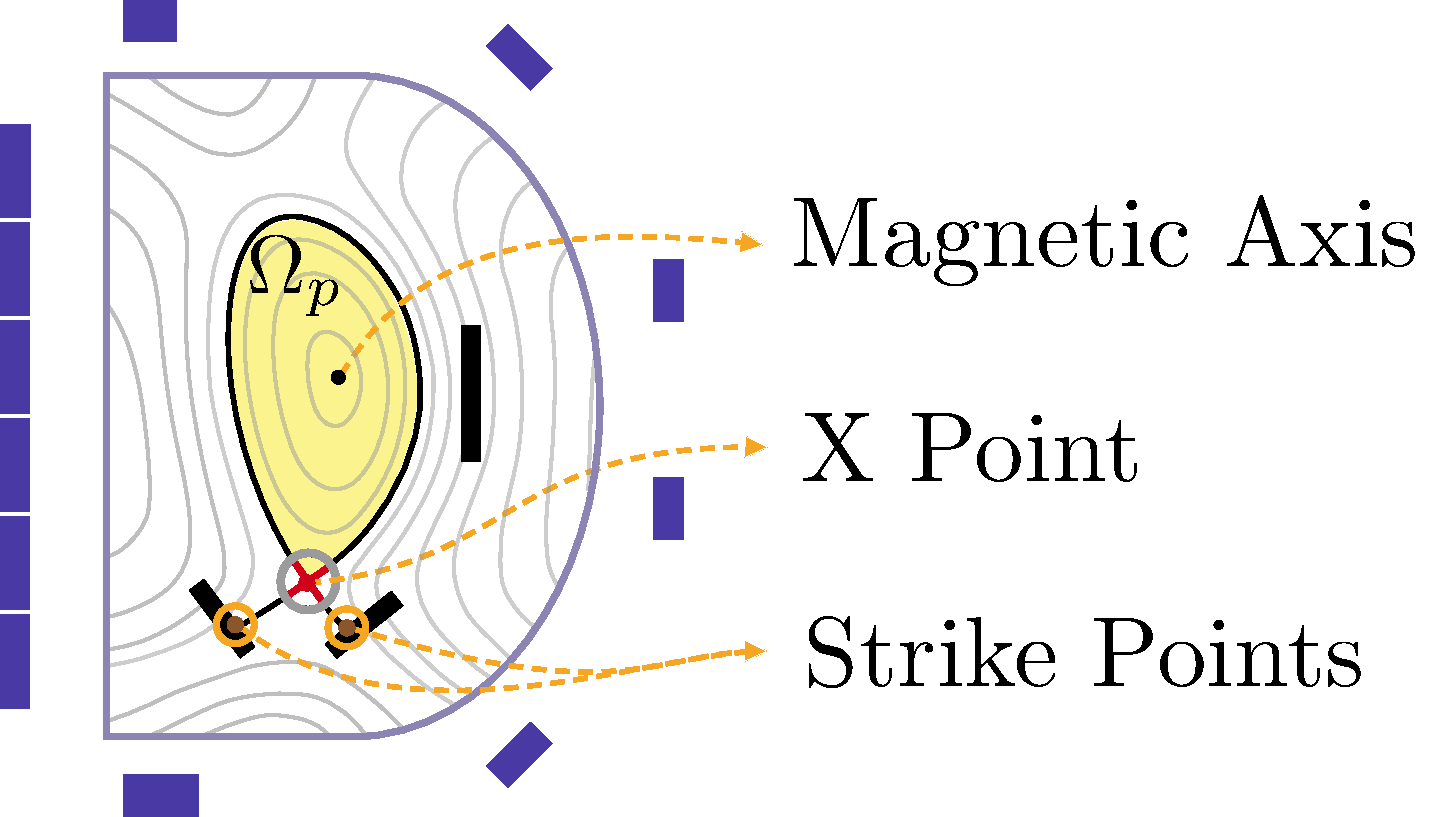
\includegraphics[height=0.45\linewidth]{StrikePoint}
            %				\caption*{Limited configuration}
        \end{subfigure}
        &
        % \hspace{-10mm}
        \begin{subfigure}{0.4\textwidth}
            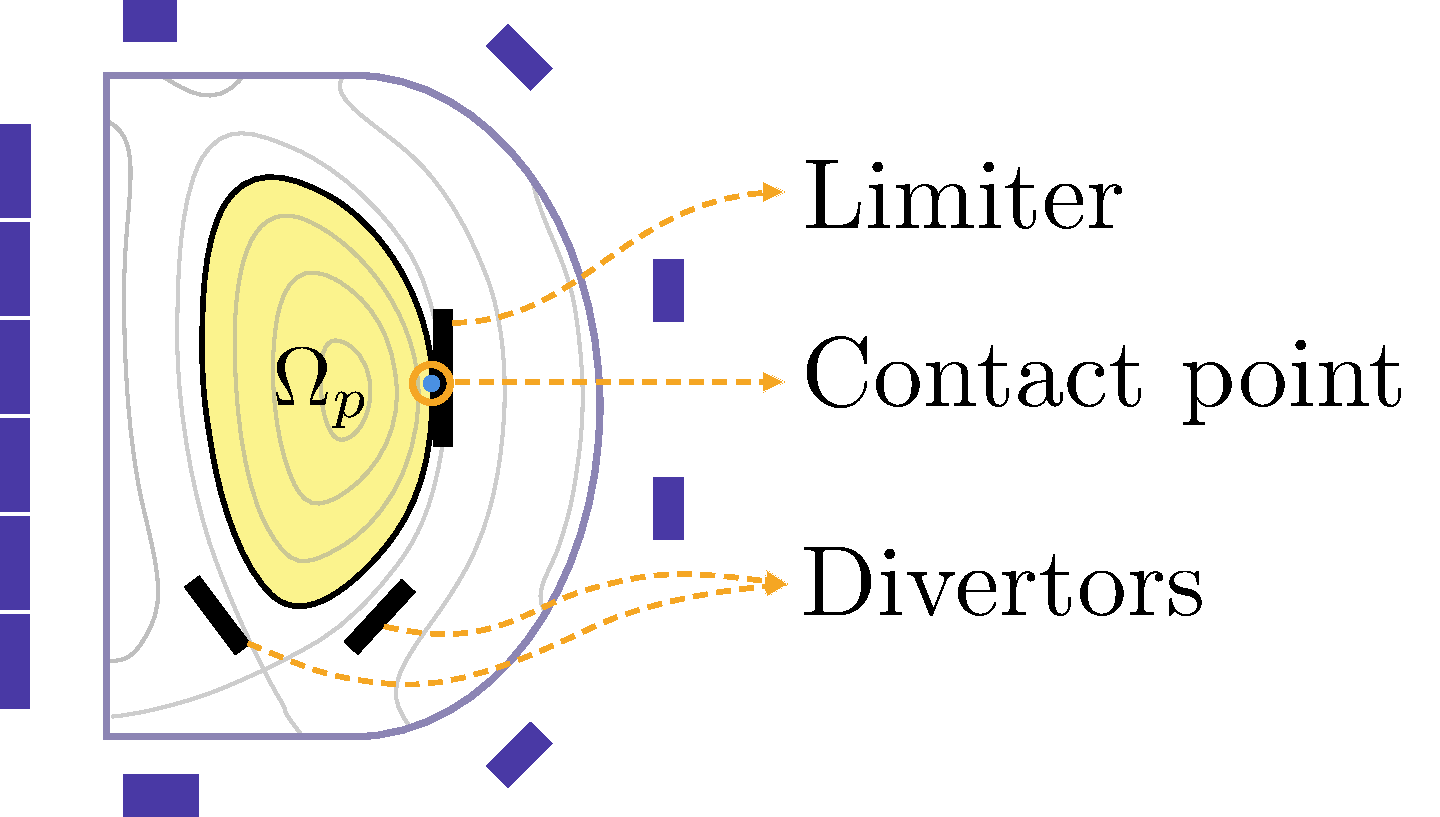
\includegraphics[height=0.45\linewidth]{ContactPoint}
            %				\caption*{Diverted configuration}
        \end{subfigure}\\
        Diverted & Limited
        
    \end{tabular}
\end{figure}


\begin{columns}[t]
\hspace{2mm} 
    \begin{column}{0.57\linewidth}
        \textcolor{myred}{\bf Diverted configuration} 

        % \vspace{1mm}
        {\footnotesize
        \begin{itemize}[leftmargin=0pt] 
            \item[$\circ$] {\bf Divertor:} A device that removes impurities.
            \item[$\circ$] {\bf Separatrix:} a boundary between closed and open field lines.
            \item[$\circ$] {\bf X-point:} saddle point of plasma field. Separatrix passes through x-point.
        \end{itemize}
        \par}
    \end{column}

    \begin{column}{0.4\linewidth}
        \textcolor{myred}{\bf Limited configuration} 
        {\footnotesize 
        \begin{itemize}[leftmargin=0pt] 
            \item[$\circ$] {\bf Limiter:} A device shields the plasma from the vacuum vessel.
            \item[$\circ$] No last closed contour line before the limiter -- {\bf Contact point}.
        \end{itemize}
        \par}
    \end{column}
\end{columns}

\end{frame}

%------------------------------------------------------------
\begin{frame}[c]
\setbeamercolor{itemize item}{fg=mygray1}
\large 	
\textcolor{mygray1}{
    \begin{itemize}[leftmargin=5pt] 
        \item[$\triangleright$]  Physical Model: Grad-Shafranov Equation
        \vspace{0.2cm}	
        \item[\textcolor{black}{$\triangleright$}] \textcolor{black}{\fontsize{25}{60}\selectfont Uncertainty Quantification}
        \vspace{0.2cm}
        \item[$\triangleright$] Objectives
        \vspace{0.2cm}
        \item[$\triangleright$] Approach 1: Surrogate-based Monte Carlo
            % \vspace{0.3cm}
            % {\footnotesize
            % \begin{itemize}[leftmargin=15pt]   
            %     \item[$\circ$] Surrogate via Sparse Grid Stochastic Collocation
            %     % \vspace{0.3cm}
            %     \item[$\circ$] Experimental Results \& Conclusions
            % \end{itemize}
            % }
        \vspace{0.2cm}
        \item[$\triangleright$] Approach 2: Multilevel Monte Carlo with Non-linear Solve
            % \vspace{0.3cm}
            % {\footnotesize
            % \begin{itemize}[leftmargin=15pt]   
            %     \item[$\circ$] Monte Carlo \& Uniform Multilevel Monte Carlo
            %     \item[$\circ$] Adaptive Multilevel Monte Carlo
            %     \item[$\circ$] Experimental Results \& Conclusions
            % \end{itemize}
            % }
        \vspace{0.2cm}
        \item[$\triangleright$] Approach 3: Surrogate-based Multilevel Monte Carlo
            % {\footnotesize
            % \begin{itemize}[leftmargin=15pt]   
            %     \item[$\circ$] Three Types of Surrogates
            %     \item[$\circ$] Surrogate-based Samplings
            %     \item[$\circ$] Experimental Results \& Conclusions
            % \end{itemize}
            % }
        \vspace{0.2cm}
        \item[$\triangleright$] Approach 4: Multi-fidelity Monte Carlo
    \end{itemize}
}
\end{frame}


%------------------------------------------------------------
\begin{frame}[t]
    \frametitle{Uncertainty Quantification (UQ)}
    \begin{itemize}[leftmargin=5pt]
        \item[$\triangleright$] \textcolor{myblue3}{\bf Source of uncertainty:} {\footnotesize Investigate the impact of \textcolor{myblue3}{uncertainties in the current intensities} on the confinement properties of a plasma.}
        
        \item[$\triangleright$] \textcolor{myred}{\bf Baseline current intensities:} 
        \[
        \footnotesize
        \begin{array}{lll}
        I_1: -1.40\times 10^6\text{A} &I_5: -9.00\times 10^6\text{A} &I_9:  -6.43\times 10^6\text{A} \\
        I_2: -9.50\times 10^6\text{A} &I_6: 3.56\times 10^6\text{A}  & I_{10}:  -4.82\times 10^6\text{A} \\
        I_3: -2.04\times 10^7\text{A} &I_7:  5.47\times 10^6\text{A}  &I_{11}:  -7.50\times 10^6\text{A} \\
        I_4: -2.04\times 10^7\text{A} &I_8: -2.27\times 10^6\text{A} &I_{12}:  1.72\times 10^7\text{A} 
        \end{array}
        \]
        \item[$\triangleright$] \textcolor{myblue3}{\bf Uncertianty Quantification:} {\footnotesize Variations in the baseline current intensities. Each current in the array is considered to be a parameter, so we have 12-dimensional parameter space.}
        
        
        \item[$\triangleright$] \textcolor{myblue3}{\bf Currents uniformly distributed:} 

        {\footnotesize
        \textcolor{mygray3}{$\tau$: perturbation level ($\tau= 1\%$ \& $2\%$). \quad $I_k$: current intensity in the $k$-th coil.}
        

        \begin{itemize}[leftmargin=15pt]   
            \item[$\circ$] Joint density function: $\displaystyle
             \pi \left(\boldsymbol{\omega}\right)=\prod_{k=1}^{d} \pi_k\left(\omega_{k}\right)=\prod_{k=1}^{d} \frac{1}{2\tau |I_k|}$.
            \item[$\circ$] 12-d parameter space: $\displaystyle W := \prod_{k=1}^{d}\left[I_k-\tau|I_k|,I_k+\tau|I_k|\right]$.
        \end{itemize}
        \par}
    \end{itemize}
\end{frame}	
% =================================================
% here I list an example of an array of currents, each current in the array is considered to be a parameter, so we have 12 dimensional parameter space, and if we use 1%...., we will use MC method to handle the uncertainty.
% =================================================



%------------------------------------------------------------
\begin{frame}[c]
\setbeamercolor{itemize item}{fg=mygray1}
\large 	
\textcolor{mygray1}{
    \begin{itemize}[leftmargin=5pt] 
        \item[$\triangleright$]  Physical Model: Grad-Shafranov Equation
        \vspace{0.2cm}	
        \item[$\triangleright$] Uncertainty Quantification
        \vspace{0.2cm}
        \item[\textcolor{black}{$\triangleright$}] \textcolor{black}{\fontsize{25}{60}\selectfont Objectives}
        \vspace{0.2cm}
        \item[$\triangleright$] Approach 1: Surrogate-based Monte Carlo
            % \vspace{0.3cm}
            % {\footnotesize
            % \begin{itemize}[leftmargin=15pt]   
            %     \item[$\circ$] Surrogate via Sparse Grid Stochastic Collocation
            %     % \vspace{0.3cm}
            %     \item[$\circ$] Experimental Results \& Conclusions
            % \end{itemize}
            % }
        \vspace{0.2cm}
        \item[$\triangleright$] Approach 2: Multilevel Monte Carlo with Non-linear Solve
            % \vspace{0.3cm}
            % {\footnotesize
            % \begin{itemize}[leftmargin=15pt]   
            %     \item[$\circ$] Monte Carlo \& Uniform Multilevel Monte Carlo
            %     \item[$\circ$] Adaptive Multilevel Monte Carlo
            %     \item[$\circ$] Experimental Results \& Conclusions
            % \end{itemize}
            % }
        \vspace{0.2cm}
        \item[$\triangleright$] Approach 3: Surrogate-based Multilevel Monte Carlo
            % {\footnotesize
            % \begin{itemize}[leftmargin=15pt]   
            %     \item[$\circ$] Three Types of Surrogates
            %     \item[$\circ$] Surrogate-based Samplings
            %     \item[$\circ$] Experimental Results \& Conclusions
            % \end{itemize}
            % }
        \vspace{0.2cm}
        \item[$\triangleright$] Approach 4: Multi-fidelity Monte Carlo
    \end{itemize}
}
\end{frame}
%------------------------------------------------------------

%------------------------------------------------------------
\begin{frame}[t]
    \frametitle{Objectives}
        \begin{itemize}[leftmargin=5pt] 
            
            \item[$\triangleright$] \textcolor{myblue3}{\bf Uncertainty Quantification} 
            
            {\fontsize{9}{9}\selectfont
            Quantify the {\bf impact of variations in current intensity} on determining 
            \begin{itemize}[leftmargin=15pt]     
                \item[\textcolor{myblue3}{$\bullet$}]   {\bf Expectation:}
                $\mathbb{E}\left[\psi(x,y,\boldsymbol \omega)\right]=\int_W \psi(x,y,\boldsymbol{\omega})\pi(\boldsymbol\omega)d\boldsymbol{\omega}.$
            
                \vspace{0.5mm}
                \item[\textcolor{myblue3}{$\bullet$}] {\bf Key plasma features:}  presence and locations of x-points, contact points, strike points \& separatrices.
                %the location where the poloidal flux function achieves saddle point
                % \item[$\circ$] \textcolor{mygray2}{Presence of strike points \& contact points.}\\

                \vspace{0.5mm}
                \item[\textcolor{myblue3}{$\bullet$}]  {\bf Geometry parameters:} elongation, triangularity etc.
                
                %						\text {Geometric parameters}
                % determint the most likely location of strike points
                % standard deviation
                %the location where the poloidal flux function achieves maximum or minimum
            \end{itemize}
            }
            \vspace{2mm}
            \item[$\triangleright$] \textcolor{myblue3}{\bf Enhancing Sampling Efficiency}
            
            {\fontsize{9}{9}\selectfont
            Use {\bf sampling methods} to approximate the expectation efficiently
            \begin{itemize}[leftmargin=15pt] 
                \vspace{2mm}
                \item[\textcolor{myblue3}{$\bullet$}] \textcolor{myblue3}{Approach 1: Surrogate-based Monte Carlo}
                
                \textcolor{mybrown1}{Replace the nonlinear solution with a {\bf surrogate function} for Monte Carlo sampling.}

                \vspace{2mm}
                \item[\textcolor{myblue3}{$\bullet$}] \textcolor{myblue3}{Approach 2: Multilevel Monte Carlo (MLMC)}
                
                \textcolor{mybrown1}{Improve efficiency by using another sampling approach -- {\bf multilevel Monte Carlo method}.}

                \vspace{2mm}
                \item[\textcolor{myblue3}{$\bullet$}] \textcolor{myblue3}{Approach 3: Surrogate-based multilevel Monte Carlo}
                
                \textcolor{mybrown1}{Further improve efficiency by using a {\bf hybrid method} that combines surrogate and multilevel Monte Carlo. }

                \vspace{2mm}
                \item[\textcolor{myblue3}{$\bullet$}] \textcolor{myblue3}{Approach 4: Multi-fidelity Monte Carlo (MFMC)}
                
                \textcolor{mybrown1}{{\bf Blending high- and low-fidelity models}, where high-fidelity models provide accuracy and low-fidelity surrogates reduce computational cost.}
            \end{itemize}
            }
    \end{itemize}
\end{frame}

% ------------------------------------------------------------
% \begin{frame}[t]
%     \frametitle{Objective}
    
%     \begin{itemize}[leftmargin=5pt]
%         \small

%         \item[$\triangleright$] \textcolor{myblue3}{\bf Goal:} Develop efficient computational algorithms to assess the impact of the current variability on the confinement properties of the plasma.
        
%         \vspace{2mm}
%         \item[$\triangleright$] This is often done by sampling methods like Monte Carlo (MC). However, it typically requires intensive and expensive nonlinear computations.

%         \vspace{2mm}
%         \item[$\triangleright$] \textcolor{myblue3}{\bf Three approaches:}
        
%             \begin{itemize}
%             \item[$\circ$] Approach 1: Surrogate-based Monte Carlo
%             \item[$\circ$] Approach 2: Multilevel Monte Carlo with the non-linear solve
%             \item[$\circ$] Approach 3: Surrogate-based multilevel Monte Carlo
%             \end{itemize}
%     \end{itemize}
% \end{frame}



%------------------------------------------------------------
\begin{frame}[c]
\setbeamercolor{itemize item}{fg=mygray1}
\large 	
\textcolor{mygray1}{
    \begin{itemize}[leftmargin=5pt] 
        \item[$\triangleright$]  Physical Model: Grad-Shafranov Equation
        \vspace{0.2cm}	
        \item[$\triangleright$] Uncertainty Quantification
        \vspace{0.2cm}
        \item[$\triangleright$]  Objectives
        \vspace{0.2cm}
        \item[\textcolor{black}{$\triangleright$}] \textcolor{black}{\fontsize{25}{60}\selectfont Approach 1: Surrogate-based Monte Carlo}
            % \vspace{0.3cm}
            % {\footnotesize
            % \begin{itemize}[leftmargin=15pt]   
            %     \item[$\circ$] Surrogate via Sparse Grid Stochastic Collocation
            %     % \vspace{0.3cm}
            %     \item[$\circ$] Experimental Results \& Conclusions
            % \end{itemize}
            % }
        \vspace{0.2cm}
        \item[$\triangleright$] Approach 2: Multilevel Monte Carlo with Non-linear Solve
            % \vspace{0.3cm}
            % {\footnotesize
            % \begin{itemize}[leftmargin=15pt]   
            %     \item[$\circ$] Monte Carlo \& Uniform Multilevel Monte Carlo
            %     \item[$\circ$] Adaptive Multilevel Monte Carlo
            %     \item[$\circ$] Experimental Results \& Conclusions
            % \end{itemize}
            % }
        \vspace{0.2cm}
        \item[$\triangleright$] Approach 3: Surrogate-based Multilevel Monte Carlo
            % {\footnotesize
            % \begin{itemize}[leftmargin=15pt]   
            %     \item[$\circ$] Three Types of Surrogates
            %     \item[$\circ$] Surrogate-based Samplings
            %     \item[$\circ$] Experimental Results \& Conclusions
            % \end{itemize}
            % }
        \vspace{0.2cm}
        \item[$\triangleright$] Approach 4: Multi-fidelity Monte Carlo
    \end{itemize}
}
\end{frame}
%------------------------------------------------------------

% %------------------------------------------------------------
\begin{frame}[t]
    \frametitle{Sparse Grid Stochastic Collocation}
\begin{itemize}[leftmargin=5pt] 

\item[$\triangleright$] Build surrogate via \textcolor{myblue3}{\bf Sparse Grid Stochastic Collocation}.
\vspace{2mm}
    \begin{itemize}[leftmargin=7pt] 
        \item [$\circ$] {\bf Idea:} {\footnotesize Select a special set of current  $\{\boldsymbol{\omega}^{(k)}\}_{1 \le k\le n_{sc}}$ in the parameter space. For each $\boldsymbol{\omega}^{(k)}$, evaluate the nonlinear solver to yield the realization $\{\psi_h^{(k)}\}$. An interpolation (surrogate) is then constructed to mimic the original nonlinear function with 
        \vspace{-3mm}
        $$\hspace{15mm}\widehat{\psi_h}(\cdot, \boldsymbol{\omega}) = \sum_k\psi_h^{(k)}(\cdot)L_{\boldsymbol{\omega}^{(k)}}(\boldsymbol{\omega}).$$
        \par}
    
        \vspace{2mm}
        \item [$\circ$] {\bf Sparse grids}: 
        \vspace{-8mm}
        \begin{figure}[H]	
        \centering
        \hspace{19mm}
        \begin{tabular}{ccc}
            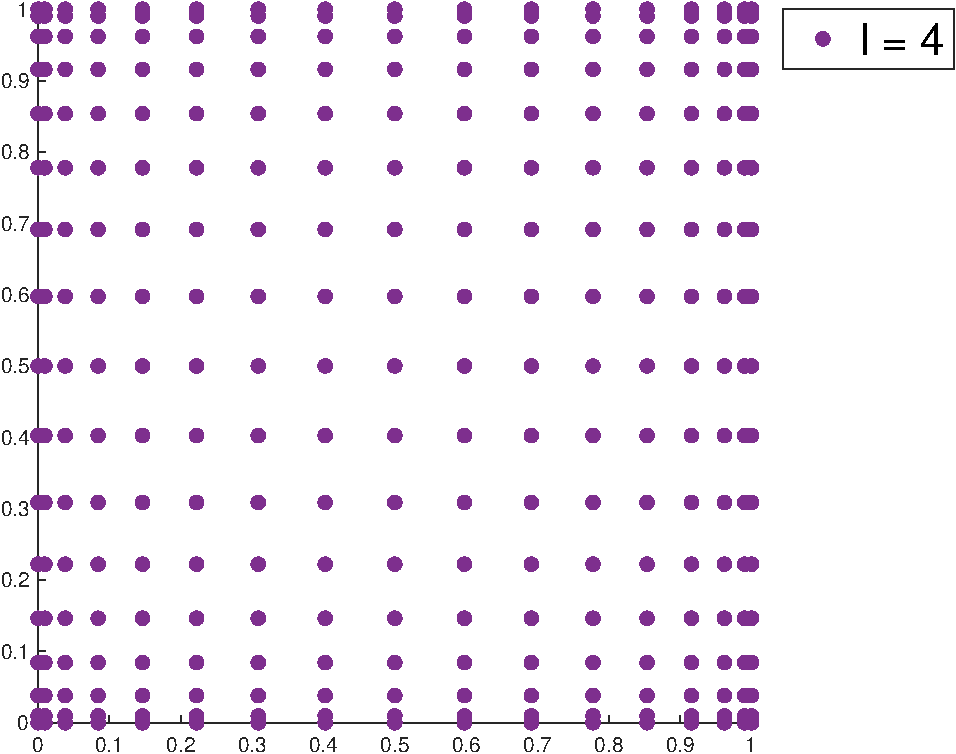
\includegraphics[width=0.2\linewidth]{full_grid_2d}
            &
            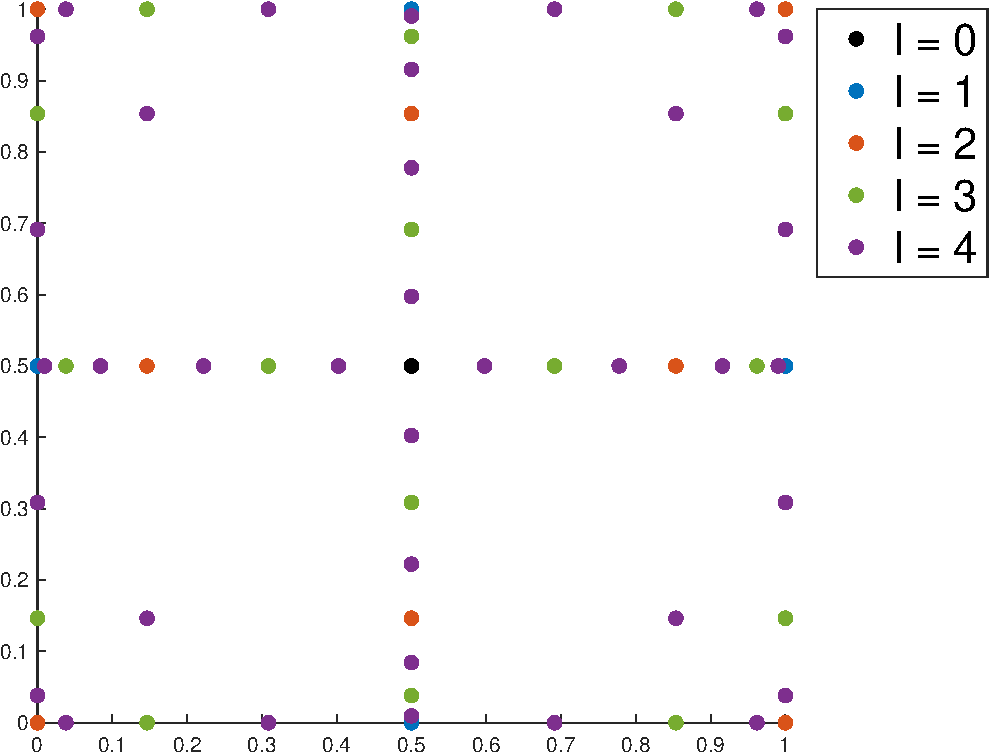
\includegraphics[width=0.2\linewidth]{sparse_grid_2d}
            &
            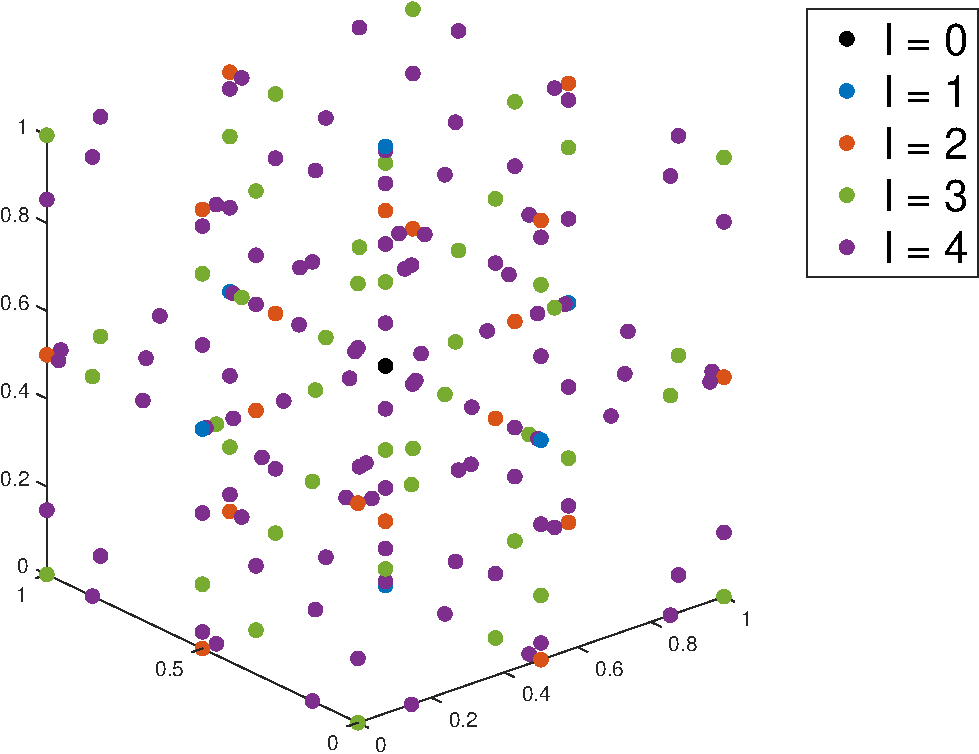
\includegraphics[width=0.2\linewidth]{sparse_grid_3d}
        \end{tabular}
        \vspace{-3mm}
        \caption*{{\fontsize{8}{8}\selectfont  Left to right: Full tensor grid 2d, level 4. Chebyshev sparse grids for 2d and 3d from level 0 to level 4. \par}}
        \end{figure}

        \vspace{-6mm}
        \fbox{%
        \parbox{1.01\textwidth}{
        \textcolor{myblue3}{\bf Theorem:} {\footnotesize Interpolation error bound in $L_\infty$ norm
        \vspace{-2mm}
        \[\|f-\mathscr{S}(f)\|_\infty = \mathscr{O}\left(N^{-k}\cdot \vert \log N\vert ^{(k+2)(d-1) +1}\right)\vspace{-2mm}\]
        $N$: \# of collocation nodes, $d$: dimension, $k$: measure of smoothness of $\psi$ wrt $\boldsymbol{\omega}$.}}}

    
        
        % {\fontsize{8}{8}\selectfont  \textcolor{mygray2}{V. Barthelmann, E. Novak, and K. Ritter. High dimensional polynomial interpolation on sparse grids. Advances in Computational Mathematics, 12:273–288, 2000.}
        % \par}

        \vspace{2mm}
        \item[$\circ$] {\bf Software:} {\footnotesize \textsc{Matlab} {\tt SPINTERP}  package -- A.Klimke.}
        
        \vspace{1mm}
        {\fontsize{8}{8}\selectfont \textcolor{mygray2}{SPINTERP, piecewise multilinear hierarchical sparse grid interpolation, http://people.math.sc.edu/burkardt/msrc/spinterp/spinterp.html, 2007.}
        \par}
        % \item [$\circ$] \textcolor{myblue3}{\bf Reference}: 
        % {\footnotesize V. Barthelmann and his collaborators.\par}
        
    
    \end{itemize}

\end{itemize}
\end{frame}
%------------------------------------------------------------
\begin{frame}[t]
    \frametitle{Approach 1: Surrogate-based Monte Carlo}
\begin{itemize}[leftmargin=5pt] 

% \item[$\triangleright$] Build surrogate via \textcolor{myblue3}{\bf Sparse Grid Stochastic Collocation}.

% \item[$\triangleright$] \textcolor{myblue3}{\bf Idea:} {\footnotesize Replace the nonlinear solve with the surrogate to perform Monte Carlo samplings.}
\item[$\triangleright$] Build surrogate via \textcolor{myblue3}{\bf Sparse Grid Stochastic Collocation}.
\item[$\triangleright$] \textcolor{myblue3}{Replace the nonlinear solve with the surrogate to perform Monte Carlo samplings.}
%
{\fontsize{7}{7}\selectfont
\begin{equation*}
\label{eq:MC_estimator}
    A^{\text{MC}}_{N} = \frac{1}{N}\sum_{i=1}^{N} \widehat \psi_{h}\left(\cdot, \boldsymbol{\omega}^{(i)}\right)
\end{equation*}
}
%
\item[$\triangleright$] \textcolor{myblue3}{\bf Efficiency:} {\footnotesize The use of surrogates reduces the CPU time required for the Monte Carlo with direct nonlinear solve by factors ranging from {\bf 7} to over {\bf 30}.}

    \vspace{-2mm}
    \begin{table}[ht]
    \centering
        \begin{threeparttable}
        \scalebox{0.55}{
        \hspace{2.4cm}
        \begin{tabular}{|c|c|c|c|c|c|c|}
        \cline{3-6}
        \multicolumn{2}{c|}{}&{\ \ Surrogate\ \ } & \ \ Surrogate \ \ &\ \ Surrogate \ \ &{\ \ Direct\ \ }\\	
        \multicolumn{2}{c|}{}&\multicolumn{1}{c|}{Level 2} &\multicolumn{1}{c|}{Level 3} &\multicolumn{1}{c|}{Level 4}
        &\multicolumn{1}{c|}{ Solver }\\
        \hline
        \multirow{3}{*}{1\% Noise}
        & \# Samples &5100&5000&5000&5200\\
        \cline{2-6}
        &Time per Sample (s.) & 0.16 & 0.59 & 3.03 & 5.22\\
        \cline{2-6}
        &Total Time (s.) &831&2944&15141&27166\\
        \hline
        \hline
        
        \multirow{3}{*}{2\% Noise}
        & \# Samples &20000&25300&31100&19100\\
        \cline{2-6}
        &Time per Sample (s.) & 0.16 & 0.59 & 3.04 & 5.69\\
        \cline{2-6}
        &Total Time (s.) &3264& 14911&94602&108620\\
        \hline
        \end{tabular}}
        \begin{tablenotes}
        \vspace{-2mm}
        {\fontsize{7}{3}\selectfont
        \item \qquad \qquad\qquad\qquad \qquad\qquad \quad\quad\quad\quad\quad\quad\quad 1 hour \quad\; 4.1 hours \quad 26 hours $\;$ 30 hours
        }
        \end{tablenotes}
        \end{threeparttable}
    \end{table}

\vspace{4mm}
    \textcolor{myred}{\bf Time saved by using surrogate:}

    \vspace{-6mm}
    \begin{table}[ht]
    \centering
    \scalebox{0.6}{
    \hspace{80mm}
        \begin{tabular}{c|c|c|}
        \cline{2-3}
        \multicolumn{1}{c|}{}&Level 2&Level 3\\
        \hline
        \multicolumn{1}{|c|}{1\% Noise}&Factor of 33&Factor of 9\\
        \hline
        \multicolumn{1}{|c|}{2\% Noise}&Factor of 33&Factor of 7\\
        \hline
        \end{tabular}}
    \end{table}

% \item[]{\bf Observation:} 
% {\footnotesize
%         \begin{itemize}[leftmargin=15pt]
%             \item[\textcolor{mygray2}{$\circ$}] \textcolor{mygray2}{Perturb all 12 currents. MC: accurate to 1\% with 95\% confidence. 
%             \item[\textcolor{mygray2}{$\circ$}] Compare average CPU times (in sec) in sampling for surrogate evaluation \& direct computation.
%             }
%         \end{itemize}
%     }

\end{itemize}
\end{frame}

%------------------------------------------------------------
\begin{frame}[t]
    \frametitle{Approach 1: Surrogate-based Monte Carlo}
\begin{itemize}[leftmargin=5pt] 


\vspace{1mm}
\item[$\triangleright$] \textcolor{myblue3}{\bf Accuracy:} 
    {\footnotesize
    Surrogate and direct non-linear solves display comparable behavior in plasma boundary and geometric descriptors, but the surrogate entails a slight compromise in accuracy.
    }
        \vspace{2mm}
        \begin{figure}[htb]\centering
        \scalebox{0.85}{
        \begin{tabular}{cccc}
        \multicolumn{2}{c}{\large{$1 \%$ current variability}} & \multicolumn{2}{c}{\large{$2 \%$ current variability}} \\ [2ex]
        \includegraphics[width=0.16\linewidth]{SurrogateLev3-Noise1} \quad&
        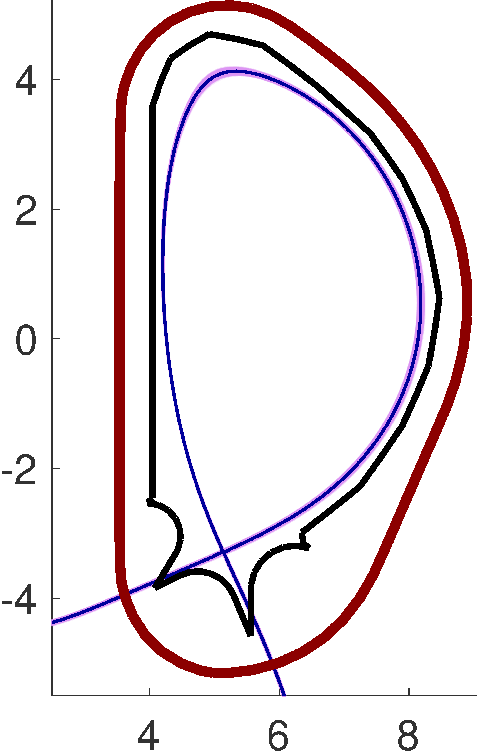
\includegraphics[width=0.16\linewidth]{DirectSolver-Noise1} \quad&
        \includegraphics[width=0.16\linewidth]{SurrogateLev3-Noise2} \quad&
        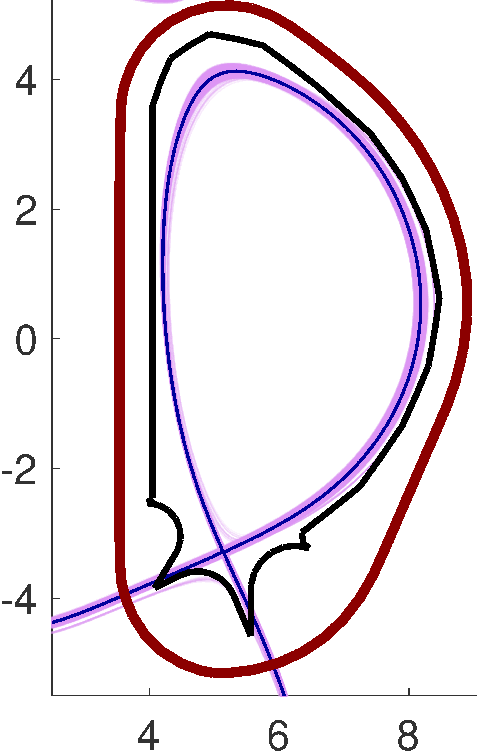
\includegraphics[width=0.16\linewidth]{DirectSolver-Noise2}\\
        {\scriptsize Surrogate level 3}& {\scriptsize Direct solution}& {\scriptsize Surrogate level 3}& {\scriptsize Direct solution}
        \end{tabular}
        }
        \end{figure}
        \vspace{2mm}
        {\fontsize{8}{8}\selectfont 
        \begin{itemize}[leftmargin=0pt]
        \item[$\circ$] Perturb all 12 currents; 2000 random samples. 
        \item[] \textcolor{myblue3}{Black \& red curves:} inner and outer walls.
        \item[] \textcolor{myblue3}{The purple region:} a union of separatrices for all 2000 samples. 
        \item[] \textcolor{myblue3}{The black line:} the separatrix of the unperturbed current. 
        
        % \item[$\circ$]
        % \item[$\circ$] The surrogate function accurately approximates the direct solver.
        \end{itemize}
        }
        \item[$\triangleright$] {\bf Reference for this project:}
        
        \vspace{0.5mm}
        {\fontsize{8}{8}\selectfont 
        \textcolor{mygray2}{H.Elman, J.Liang, T.Sánchez-Vizuet. Surrogate approximation of the Grad-Shafranov free boundary problem via stochastic collocation on sparse grids. JCP, 448 (2022).}
        \par}
\end{itemize}
\end{frame}


%------------------------------------------------------------
\begin{frame}[c]
\setbeamercolor{itemize item}{fg=mygray1}
\large 	
\textcolor{mygray1}{
    \begin{itemize}[leftmargin=5pt] 
        \item[$\triangleright$]  Physical Model: Grad-Shafranov Equation
        \vspace{0.2cm}	
        \item[$\triangleright$] Uncertainty Quantification
        \vspace{0.2cm}
        \item[$\triangleright$]  Objectives
        \vspace{0.2cm}
        \item[$\triangleright$] Approach 1: Surrogate-based Monte Carlo
            % \vspace{0.3cm}
            % {\footnotesize
            % \begin{itemize}[leftmargin=15pt]   
            %     \item[$\circ$] Surrogate via Sparse Grid Stochastic Collocation
            %     % \vspace{0.3cm}
            %     \item[$\circ$] Experimental Results \& Conclusions
            % \end{itemize}
            % }
        \vspace{0.2cm}
        \item[\textcolor{black}{$\triangleright$}] \textcolor{black}{\fontsize{25}{60}\selectfont Approach 2: Multilevel Monte Carlo with Non-linear Solve}
            % \vspace{0.3cm}
            % {\footnotesize
            % \begin{itemize}[leftmargin=15pt]   
            %     \item[$\circ$] Monte Carlo \& Uniform Multilevel Monte Carlo
            %     \item[$\circ$] Adaptive Multilevel Monte Carlo
            %     \item[$\circ$] Experimental Results \& Conclusions
            % \end{itemize}
            % }
        \vspace{0.2cm}
        \item[$\triangleright$] Approach 3: Surrogate-based Multilevel Monte Carlo
            % {\footnotesize
            % \begin{itemize}[leftmargin=15pt]   
            %     \item[$\circ$] Three Types of Surrogates
            %     \item[$\circ$] Surrogate-based Samplings
            %     \item[$\circ$] Experimental Results \& Conclusions
            % \end{itemize}
            % }
        \vspace{0.2cm}
        \item[$\triangleright$] Approach 4: Multi-fidelity Monte Carlo
    \end{itemize}
}
\end{frame}
%------------------------------------------------------------



%------------------------------------------------------------
\begin{frame}[t]
    \frametitle{Approach 2: Multilevel Monte Carlo with Non-linear Solve}
\begin{itemize}[leftmargin=5pt] 

\item[$\triangleright$] \textcolor{myblue3}{\bf Multilevel Monte Carlo:} {\footnotesize Reduce sampling costs by  focusing most of the work on coarser grids rather than fine grids,  which are typically used in standard Monte Carlo simulations.}
\vspace{-2mm}
{\fontsize{7}{7}\selectfont 
\begin{equation*}
% \label{eq:MFMC_estimator_independent}
    A^{\text{MLMC}} = A^{\text{MC}}_{L,N_L} +  \sum_{k=1}^{L-1} \left(A_{k,N_{k}}^{\text{MC}}- A_{k-1,N_k}^{\text{MC}}\right) 
\end{equation*}

\vspace{-1mm}
$A_{k,N_{k}}^{\text{MC}}\;\; \& \;\; A_{k-1,N_k}^{\text{MC}}$ uses same samples across different resolution levels.
}

% \vspace{-2mm}
{\fontsize{7}{7}\selectfont \textcolor{mygray2}{M. B. Giles. Multilevel Monte Carlo methods. Acta Numer., 24:259–328, 2015.}\par}

\vspace{2mm}
\begin{itemize}[leftmargin=7pt] 
% \item [$\circ$] {\bf MLMC estimator:}  
%     \vspace{-8mm}
%     {\fontsize{6.8}{6.8}\selectfont 
%         \[
%         \hspace{30mm}
%         A_{\text{MLMC}}:= \mathbb{E}(u_L)= \frac{1}{N_0}\sum_{i = 1}^{N_0}u_{0}^{(i)}+\sum_{\ell=1}^L \frac{1}{N_\ell}\sum_{i=1}^{N_\ell}\left(u_{\ell}^{(i)}-u_{\ell-1}^{(i)}\right),
%         % \vspace{-2mm}
%         \]
%     }
    % {\footnotesize
    % \textcolor{mygray2}{$u_\ell$: Discretized solution with mesh parameter $h_\ell$.}
    
    %     \textcolor{mygray2}{$L$: \# of mesh levels. $\quad\quad$ $N_\ell$: \# of samples on mesh level $\ell$.}
    % }
    
\item [$\circ$] {\bf Generation of uniform meshes: }
{\footnotesize
\begin{itemize}[leftmargin=15pt]
\item[$\star$]  {\fontsize{9}{9}\selectfont \textcolor{myred}{Geometry-conforming meshes} -- tailored to the curved boundaries of the mesh geometry, \textcolor{myred}{non-nested}.\par}
\end{itemize}
}

\vspace{2mm}
\begin{figure}[h!]\centering
\scalebox{0.7}{
\begin{tabular}{ccc}
    \hspace{-5mm}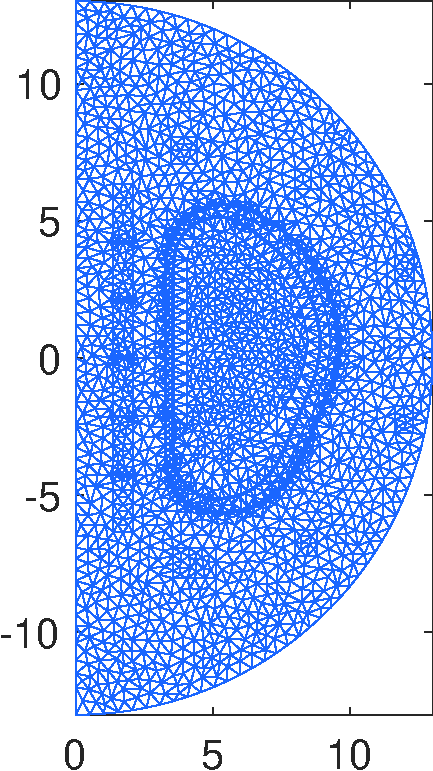
\includegraphics[width=0.2\linewidth]{Mesh_Coarse_x2.pdf}&
    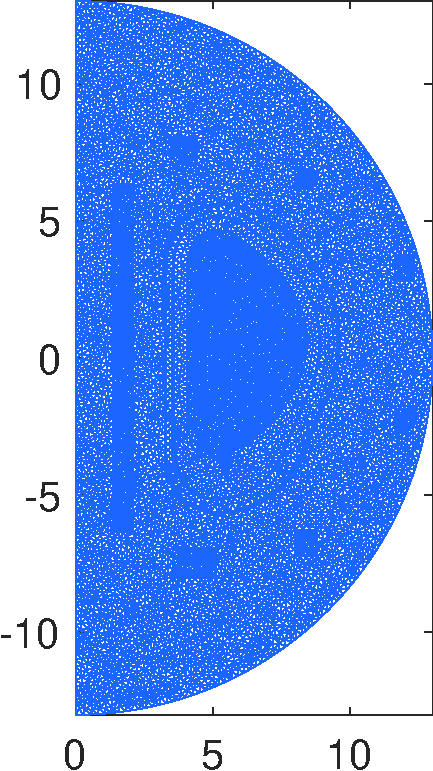
\includegraphics[width=0.2\linewidth]{Mesh_Coarse_x1.pdf}&
    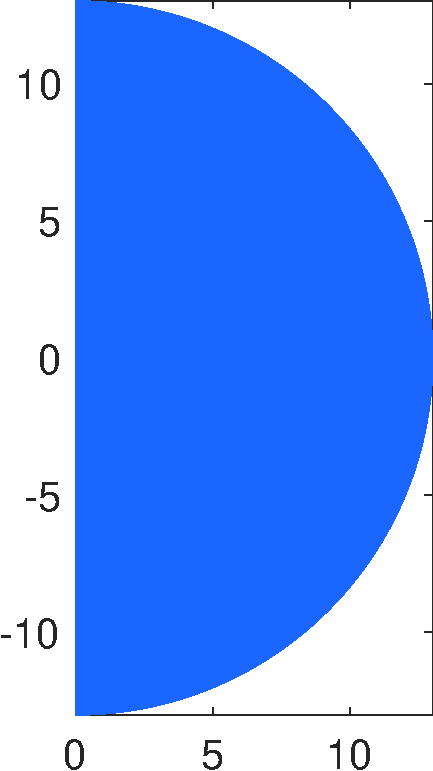
\includegraphics[width=0.2\linewidth]{Mesh_Ref.pdf}\\
    % \includegraphics[width=0.2\linewidth]{Mesh_Adapt3.pdf}\\
    $\ell=0$&$\ell=1$&$\ell=2$\\
\end{tabular}
%	\caption{Three uniformly refined geometric conforming meshes ($\ell=0,3,6,7$) for MLMC simulation.} 
%	\label{fig:Exp_result}
% \vspace{-3mm}
}
\end{figure}
\item[$\circ$] {\bf Generation of deterministic adaptive refined grids: }
        {\footnotesize
        \begin{itemize}[leftmargin=15pt]
            
            % \vspace{2mm}
            \item[$\star$] {\fontsize{9}{9}\selectfont Start from the same coarsest mesh as the uniform mesh. Using an $L_2$ a posteriori error estimator and D\"{o}rfler marking strategy. Select a sequence of adaptively refined meshes with error decay $1/4$. \textcolor{myred}{nested}.\par}
        
            % \item[$\triangleright$]  
        \end{itemize}
        \par}
\end{itemize}
% \item[$\triangleright$] \textcolor{myblue3}{\bf Efficiency:} 
\end{itemize}
\end{frame}




%------------------------------------------------------------
\begin{frame}[t]
    \frametitle{Approach 2: Multilevel Monte Carlo with Non-linear Solve}
\begin{itemize}[leftmargin=5pt] 
\item[$\triangleright$] \textcolor{myblue3}{\bf Efficiency:} {\footnotesize Multilevel Monte Carlo reduces CPU time for Monte Carlo sampling by factors of {\bf 60} to over {\bf 200}. Both uniform and adaptive MLMC achieve comparable sampling costs.}
\vspace{2mm}
\begin{figure}[ht!]\centering
\scalebox{0.9}{
\begin{tabular}{cc}
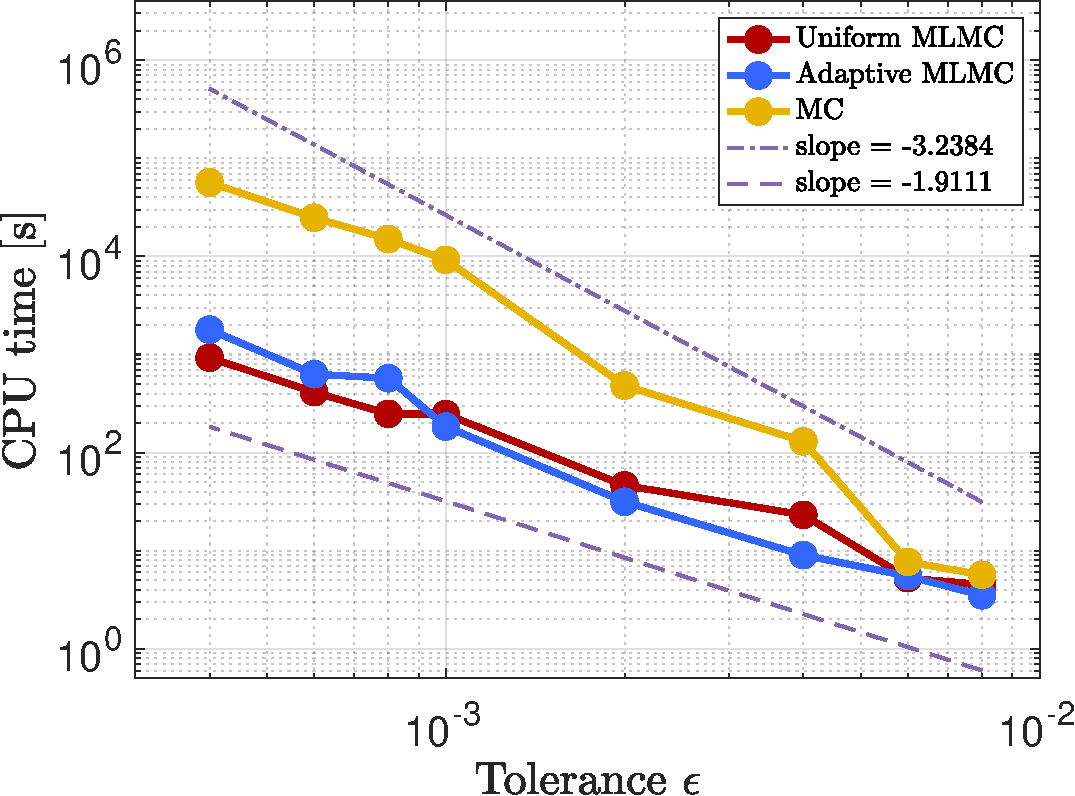
\includegraphics[height=0.4\linewidth]{CPUtime_epsilon_L2norm.pdf}&
% 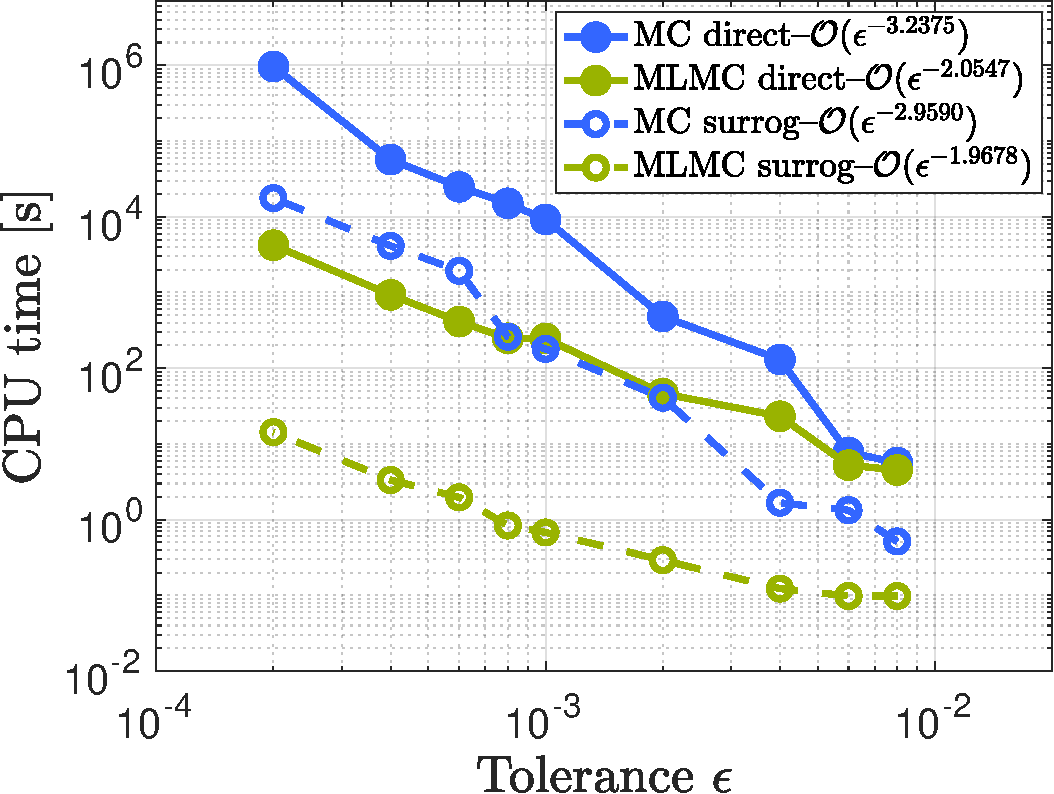
\includegraphics[height=0.35\linewidth]{CPUtime_direct_n_surrog_coil1_12.pdf}
\end{tabular}
}
% \caption{Left: sampling cost (CPU time in seconds) of direct computation vs. tolerance $\epsilon$ for MC, MLMC with geometry-conforming uniform meshes, and MLMC with adaptive meshes.  Right: sampling cost vs. tolerance $\epsilon$ for MC with both direct computation and surrogate, MLMC with both direct computation and surrogate.} 
\label{fig:Experiment_result_plot}
\end{figure}

\end{itemize}
\end{frame}



%------------------------------------------------------------
\begin{frame}[t]
    \frametitle{Approach 2: Multilevel Monte Carlo with Non-linear Solve}
\begin{itemize}[leftmargin=5pt] 

\item[$\triangleright$] \textcolor{myblue3}{\bf Accuracy:} 
{\footnotesize
\begin{itemize}[leftmargin=5pt] 
    \item[$\circ$] Compared to MC, uniform MLMC exhibits significant plasma boundary distortion due to extrapolation error on non-nested meshes. 
    \item[$\circ$] As a remedy, we interpolate correction terms from coarse meshes to a fine common mesh. However, this improves accuracy but reduces efficiency.
    \item[$\circ$] In contrast, adaptive gridding is more effective in yielding accurate geometric quantities.
\end{itemize}
}


\vspace{-4mm}
\begin{figure}[ht!]\centering
% \scalebox{1}{
\begin{tabular}{cc}
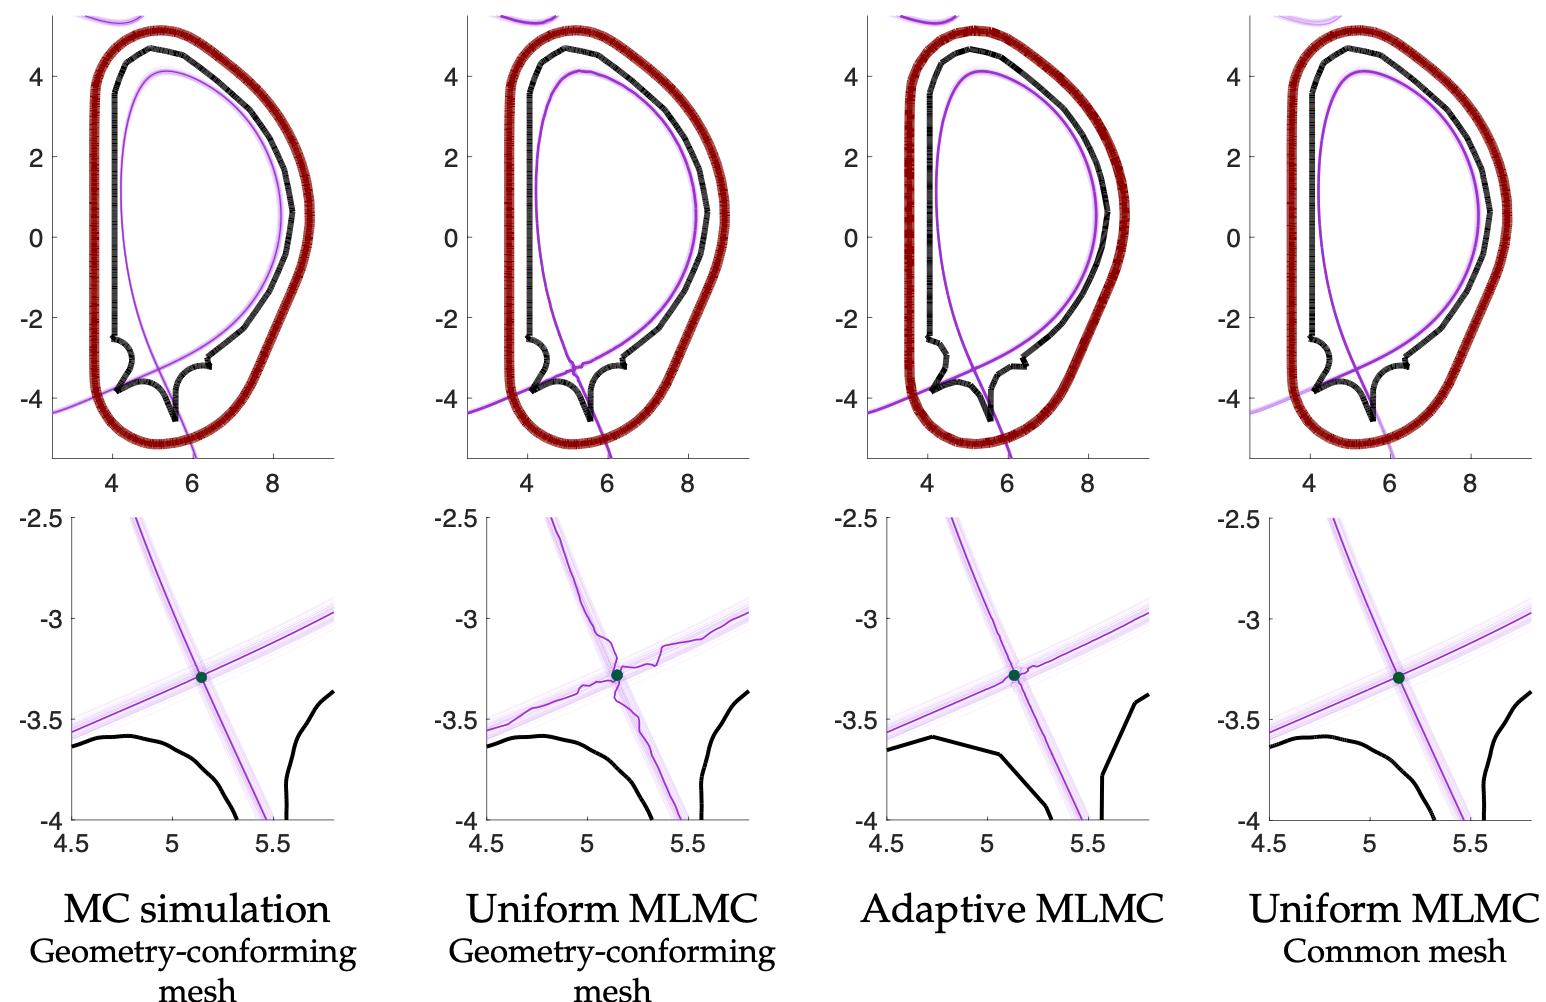
\includegraphics[height=0.4\linewidth]{Figure2.png}
\end{tabular}
% }
\end{figure}

% \vspace{-2mm}
% \begin{itemize}[leftmargin=5pt]
%     \item[$\triangleright$] \textcolor{myblue3}{\bf The behaviors of separatrices near the x-point:}

% \end{itemize}

\item[$\triangleright$] {\bf Reference for this project:}
% \vspace{-1mm}
        
{\fontsize{8}{8}\selectfont \textcolor{mygray2}{H.Elman, J.Liang, T.Sánchez-Vizuet. Multilevel Monte Carlo methods for the Grad-Shafranov free boundary problem. CPC, 298 (2024).}
\par}
\end{itemize}
\end{frame}




%------------------------------------------------------------
\begin{frame}[c]
\setbeamercolor{itemize item}{fg=mygray1}
\large 	
\textcolor{mygray1}{
    \begin{itemize}[leftmargin=5pt] 
        \item[$\triangleright$]  Physical Model: Grad-Shafranov Equation
        \vspace{0.2cm}	
        \item[$\triangleright$] Uncertainty Quantification
        \vspace{0.2cm}
        \item[$\triangleright$]  Objectives
        \vspace{0.2cm}
        \item[$\triangleright$]  Approach 1: Surrogate-based Monte Carlo
            % \vspace{0.3cm}
            % {\footnotesize
            % \begin{itemize}[leftmargin=15pt]   
            %     \item[$\circ$] Surrogate via Sparse Grid Stochastic Collocation
            %     % \vspace{0.3cm}
            %     \item[$\circ$] Experimental Results \& Conclusions
            % \end{itemize}
            % }
        \vspace{0.2cm}
        \item[$\triangleright$] Approach 2: Multilevel Monte Carlo with Non-linear Solve
            % \vspace{0.3cm}
            % {\footnotesize
            % \begin{itemize}[leftmargin=15pt]   
            %     \item[$\circ$] Monte Carlo \& Uniform Multilevel Monte Carlo
            %     \item[$\circ$] Adaptive Multilevel Monte Carlo
            %     \item[$\circ$] Experimental Results \& Conclusions
            % \end{itemize}
            % }
        \vspace{0.2cm}
        \item[\textcolor{black}{$\triangleright$}] \textcolor{black}{\fontsize{25}{60}\selectfont Approach 3: Surrogate-based Multilevel Monte Carlo}
            % {\footnotesize
            % \begin{itemize}[leftmargin=15pt]   
            %     \item[$\circ$] Three Types of Surrogates
            %     \item[$\circ$] Surrogate-based Samplings
            %     \item[$\circ$] Experimental Results \& Conclusions
            % \end{itemize}
            % }
        \vspace{0.2cm}
        \item[$\triangleright$] Approach 4: Multi-fidelity Monte Carlo
    \end{itemize}
}
\end{frame}
%------------------------------------------------------------


%------------------------------------------------------------
\begin{frame}[t]
    \frametitle{Approach 3: Surrogate-based Multilevel Monte Carlo}
\begin{itemize}[leftmargin=5pt] 
% \item[$\triangleright$] \textcolor{myblue3}{\bf Surrogate-enhanced multilevel Monte Carlo:} {\footnotesize Integrate surrogate with multilevel Monte Carlo.}
\item[$\triangleright$] \textcolor{myblue3}{\bf Surrogate-enhanced multilevel Monte Carlo:} {\footnotesize Integrate surrogate with multilevel Monte Carlo.}
\item[$\triangleright$] \textcolor{myblue3}{\bf Efficiency:} {\footnotesize 
 Surrogate-based multilevel Monte Carlo significantly diminishes the cost of direct nonlinear solve by a factor ranging from {\bf 50} to {\bf 300}. In comparison to MC with direct non-linear solve, this approach manifests a dramatic speedup ranging from {\bf 60} to $\boldsymbol{6\times 10^4}$.}
 \vspace{3mm}
\begin{figure}[ht!]\centering
\scalebox{0.9}{
\begin{tabular}{cc}
% 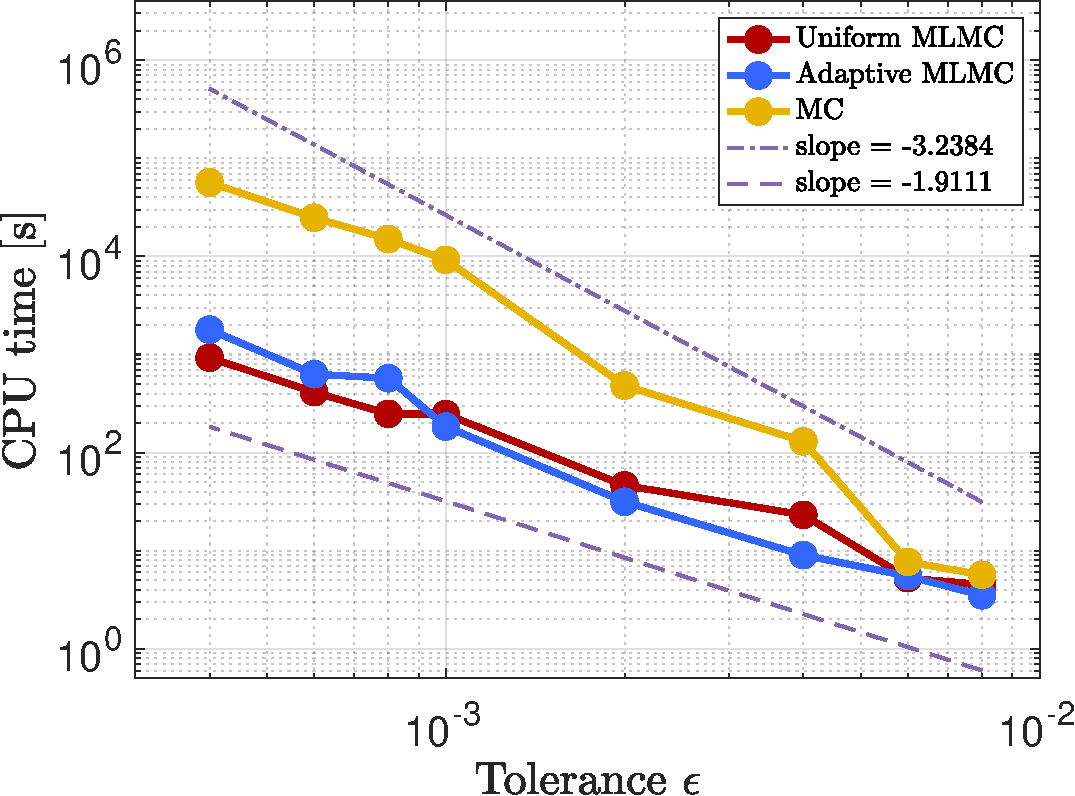
\includegraphics[height=0.35\linewidth]{CPUtime_epsilon_L2norm.pdf}&
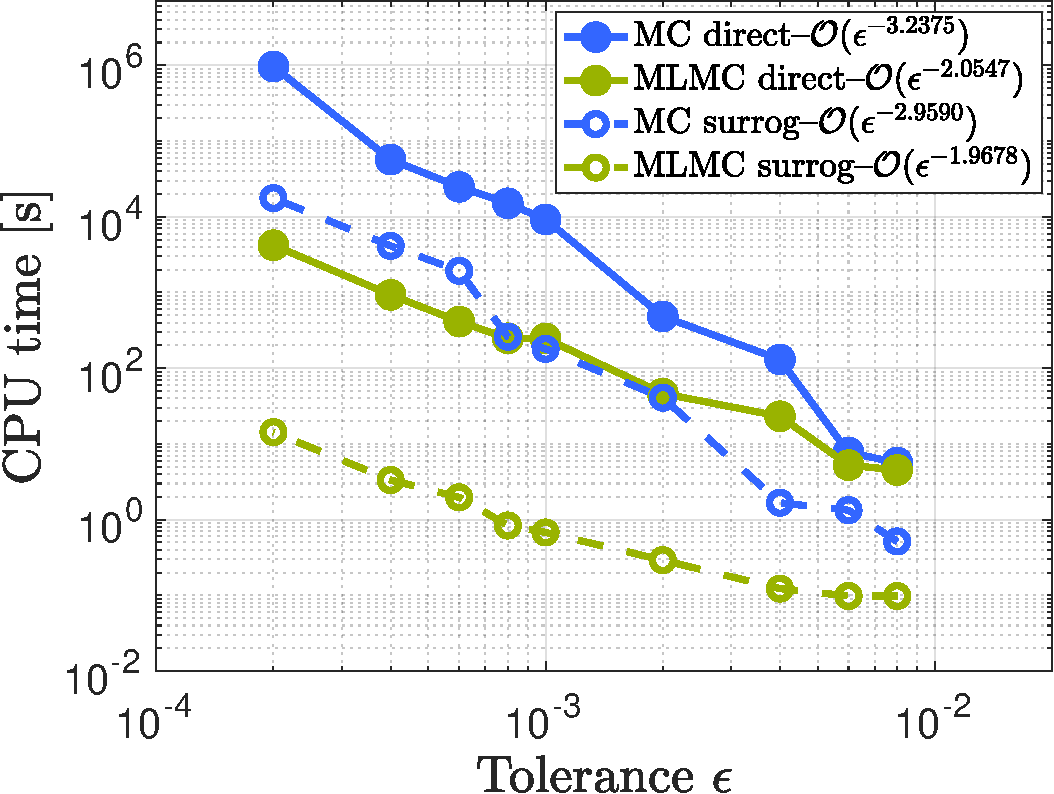
\includegraphics[height=0.4\linewidth]{CPUtime_direct_n_surrog_coil1_12.pdf}
\end{tabular}
}
% \caption{Left: sampling cost (CPU time in seconds) of direct computation vs. tolerance $\epsilon$ for MC, MLMC with geometry-conforming uniform meshes, and MLMC with adaptive meshes.  Right: sampling cost vs. tolerance $\epsilon$ for MC with both direct computation and surrogate, MLMC with both direct computation and surrogate.} 
\label{fig:Experiment_result_plot}
\end{figure}

\end{itemize}
\end{frame}
 
%------------------------------------------------------------
\begin{frame}[t]
    \frametitle{Approach 3: Surrogate-based Multilevel Monte Carlo}
\begin{itemize}[leftmargin=5pt] 

\item[$\triangleright$] \textcolor{myblue3}{\bf Accuracy:} {\footnotesize Plasma boundary and geometric descriptors obtained through surrogate-based MLMC samplings exhibit similar behavior compared to their direct non-linear solve counterparts.}
 % \vspace{3mm}
\begin{figure}[ht!]\centering
\scalebox{0.15}{
\begin{tabular}{cccc}
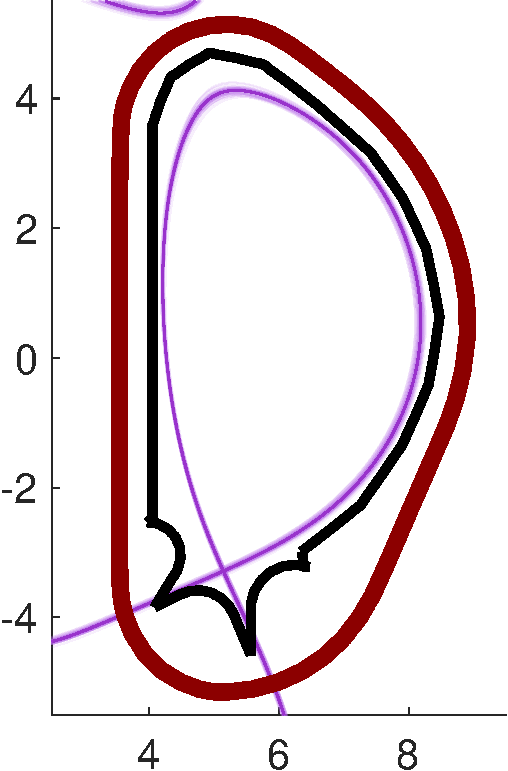
\includegraphics[width=1\linewidth]{QoI_MC_uniform.pdf}
&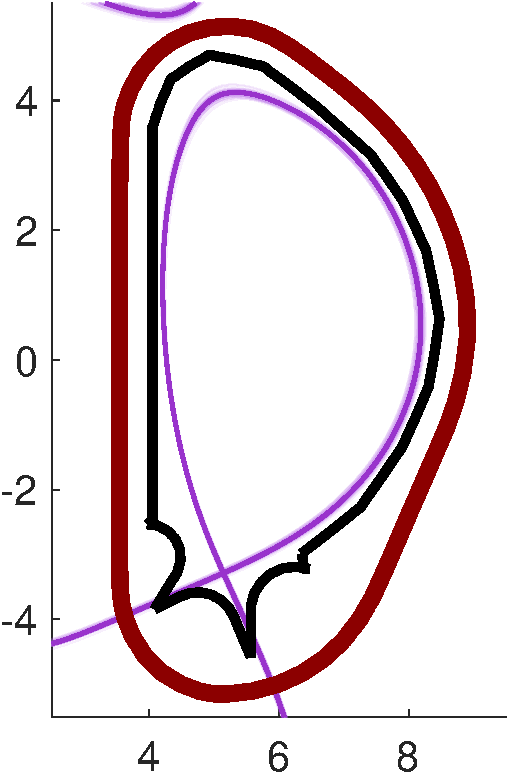
\includegraphics[width=1\linewidth]{QoI_MC_surrogate.pdf}
&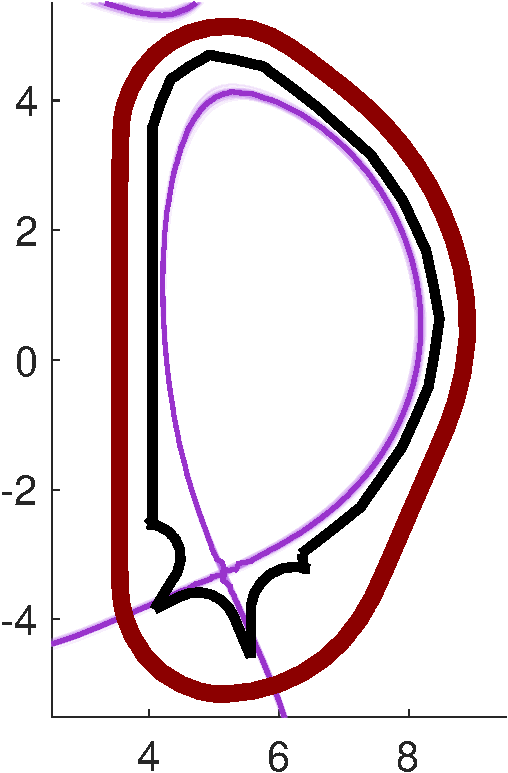
\includegraphics[width=1\linewidth]{QoI_MLMC_uniform_L2norm.pdf} 
&\includegraphics[width=1\linewidth]{QoI_MLMC_surrogate.pdf} 
% &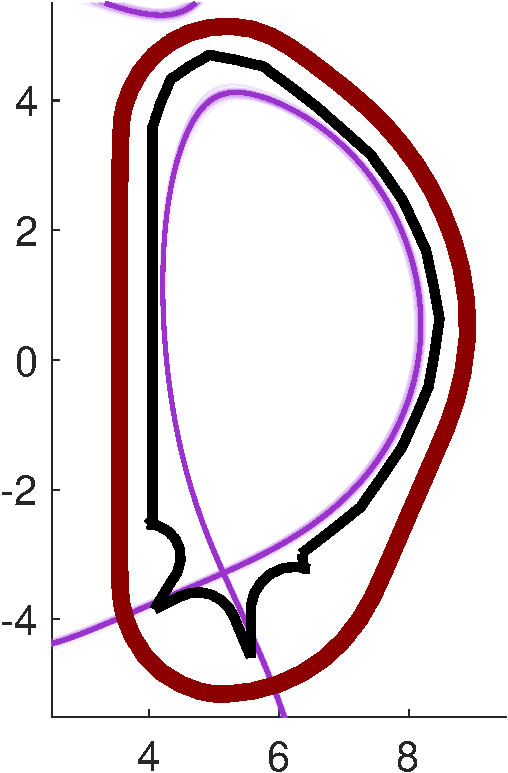
\includegraphics[width=1\linewidth]{QoI_MLMC_DirectSolver_Interp2CommonGrid.pdf} 
% &\includegraphics[width=1\linewidth]{QoI_MLMC_surrogate_Interp2CommonGrid.pdf} 
\\
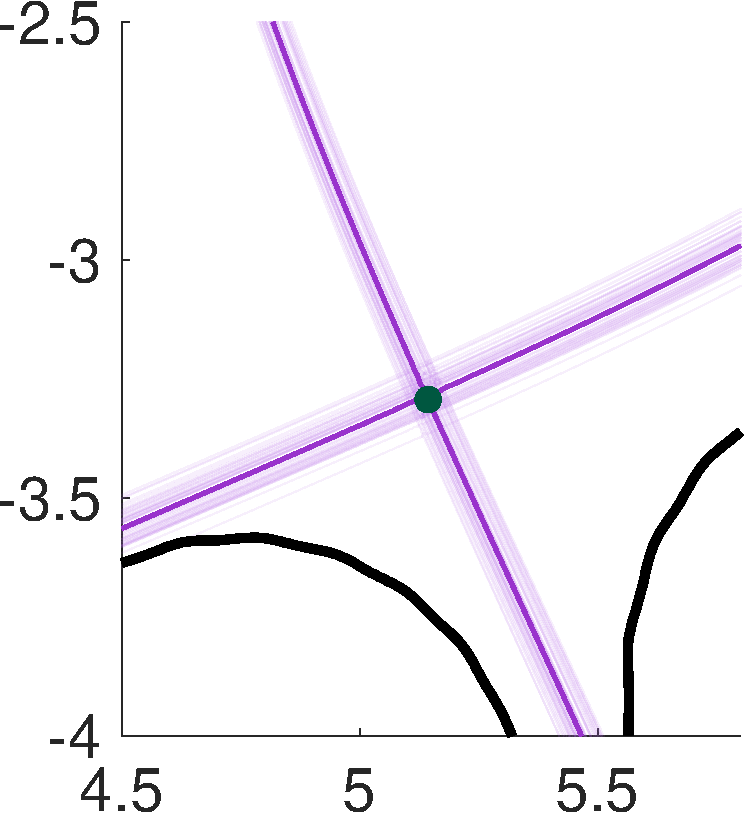
\includegraphics[width=1\linewidth]{QoI_MC_uniform_xptRegion.pdf} 
&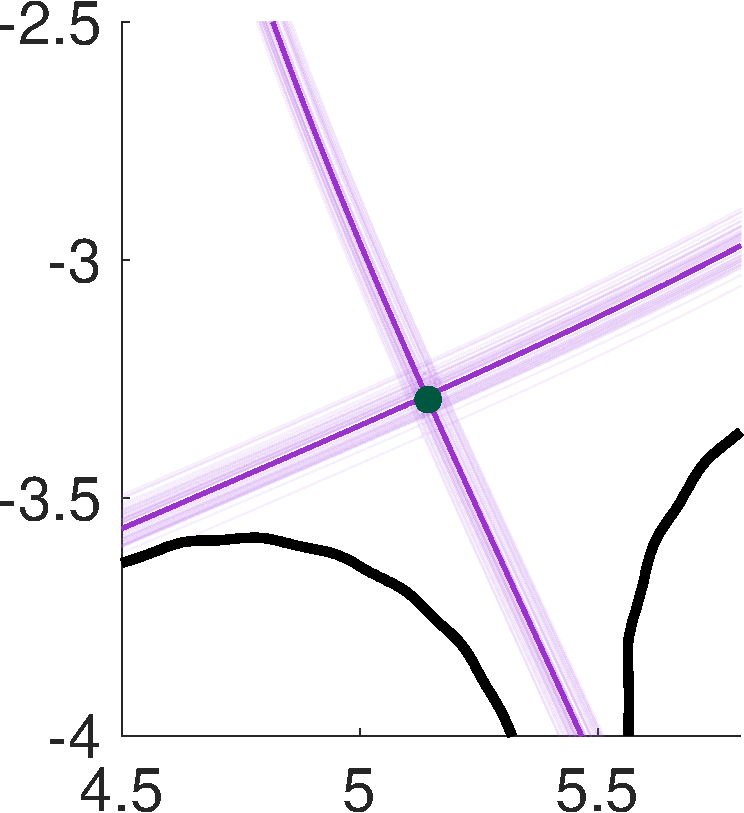
\includegraphics[width=1\linewidth]{QoI_MC_surrogate_xptRegion.pdf}
&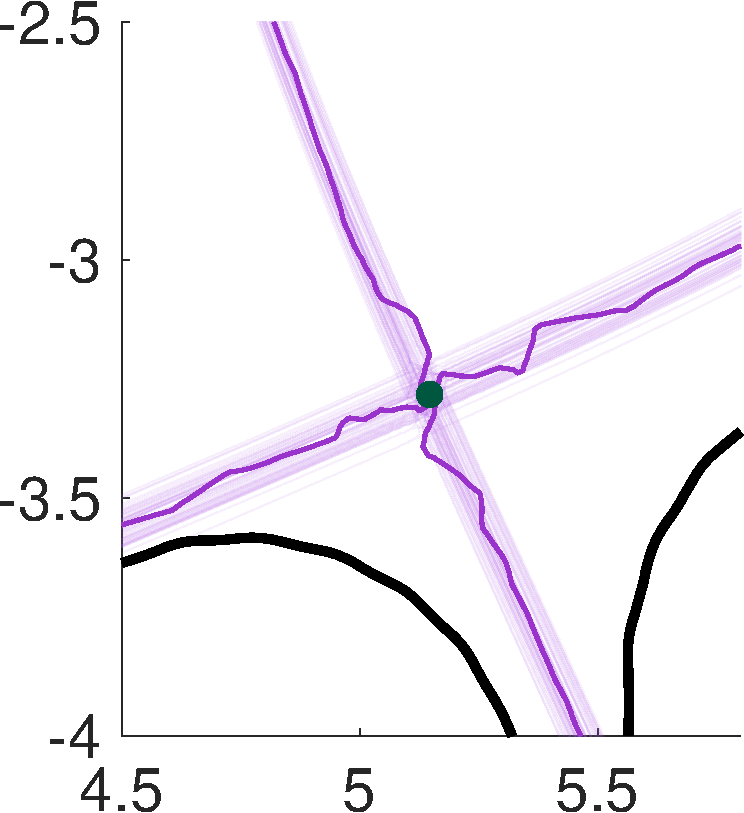
\includegraphics[width=1\linewidth]{QoI_MLMC_uniform_xptRegion_L2norm.pdf} 
&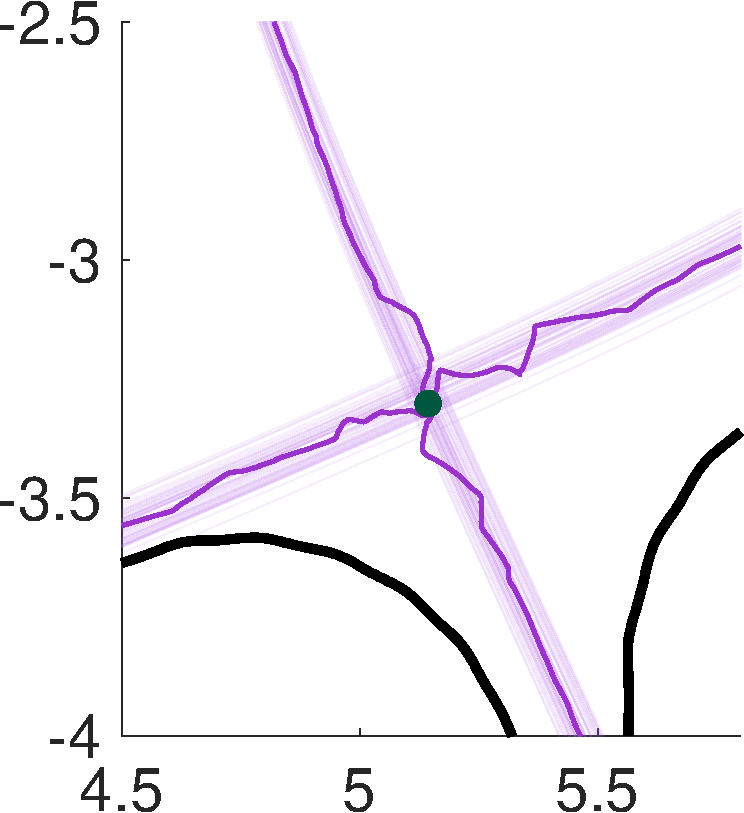
\includegraphics[width=1\linewidth]{QoI_MLMC_surrogate_xptRegion.pdf} 
% &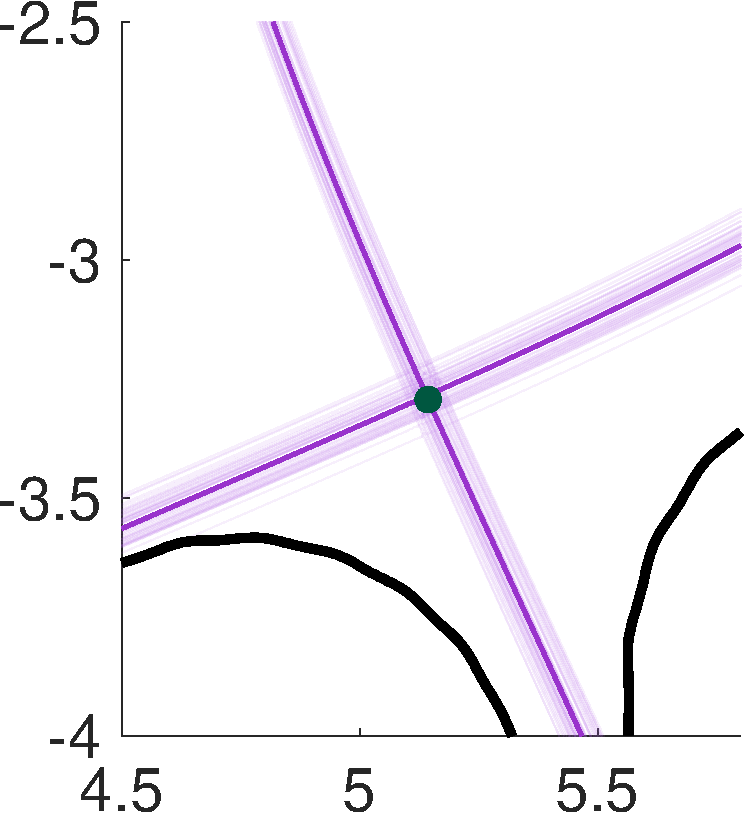
\includegraphics[width=1\linewidth]{QoI_MLMC_DirectSolver_xptRegion_Interp2CommonGrid.pdf}
% &\includegraphics[width=1\linewidth]{QoI_MLMC_surrogate_xptRegion_Interp2CommonGrid.pdf}
\\[1ex]
\quad {\fontsize{35}{35}\selectfont MC + Direct} & {\fontsize{35}{35}\selectfont MC + Surrogate}  &{\fontsize{35}{35}\selectfont MLMC + Direct} &{\fontsize{35}{35}\selectfont MLMC + Surrogate} 
% & {\fontsize{35}{35}\selectfont MLMC + Direct + interp} 
% &{\fontsize{35}{35}\selectfont MLMC + Surrogate + interp} 
\\[-0.5ex]
\end{tabular}
}
\end{figure}

%
\vspace{1mm}
\item[$\triangleright$] {\bf Reference for this project:}
\vspace{1mm}
        
{\fontsize{8}{8}\selectfont \textcolor{mygray2}{H.Elman, J.Liang, T.Sánchez-Vizuet., Surrogate-based multilevel Monte Carlo methods for uncertainty quantification in the Grad-Shafranov free boundary problem, https://arxiv.org/abs/2501.08482.}
\par}
\end{itemize}
\end{frame}


%------------------------------------------------------------
\begin{frame}[c]
\setbeamercolor{itemize item}{fg=mygray1}
\large 	
\textcolor{mygray1}{
    \begin{itemize}[leftmargin=5pt] 
        \item[$\triangleright$]  Physical Model: Grad-Shafranov Equation
        \vspace{0.2cm}	
        \item[$\triangleright$] Uncertainty Quantification
        \vspace{0.2cm}
        \item[$\triangleright$]  Objectives
        \vspace{0.2cm}
        \item[$\triangleright$]  Approach 1: Surrogate-based Monte Carlo
            % \vspace{0.3cm}
            % {\footnotesize
            % \begin{itemize}[leftmargin=15pt]   
            %     \item[$\circ$] Surrogate via Sparse Grid Stochastic Collocation
            %     % \vspace{0.3cm}
            %     \item[$\circ$] Experimental Results \& Conclusions
            % \end{itemize}
            % }
        \vspace{0.2cm}
        \item[$\triangleright$] Approach 2: Multilevel Monte Carlo with Non-linear Solve
            % \vspace{0.3cm}
            % {\footnotesize
            % \begin{itemize}[leftmargin=15pt]   
            %     \item[$\circ$] Monte Carlo \& Uniform Multilevel Monte Carlo
            %     \item[$\circ$] Adaptive Multilevel Monte Carlo
            %     \item[$\circ$] Experimental Results \& Conclusions
            % \end{itemize}
            % }
        \vspace{0.2cm}
        \item[$\triangleright$]  Approach 3: Surrogate-based Multilevel Monte Carlo
            % {\footnotesize
            % \begin{itemize}[leftmargin=15pt]   
            %     \item[$\circ$] Three Types of Surrogates
            %     \item[$\circ$] Surrogate-based Samplings
            %     \item[$\circ$] Experimental Results \& Conclusions
            % \end{itemize}
            % }
        \vspace{0.2cm}
        \item[\textcolor{black}{$\triangleright$}] \textcolor{black}{\fontsize{25}{60}\selectfont Approach 4: Multi-fidelity Monte Carlo}
    \end{itemize}
}
\end{frame}
%------------------------------------------------------------

%------------------------------------------------------------
\begin{frame}[t]
    \frametitle{Approach 4: Multi-fidelity Monte Carlo}
\begin{itemize}[leftmargin=5pt] 
% \item[$\triangleright$] \textcolor{myblue3}{\bf Surrogate-enhanced multilevel Monte Carlo:} {\footnotesize Integrate surrogate with multilevel Monte Carlo.}
\item[$\triangleright$] \textcolor{myblue3}{\bf Multi-fidelity Monte Carlo} 

{\footnotesize A variance reduction technique that efficiently estimates statistical quantities by fusing high-fidelity and low-fidelity models, maintaining accuracy while significantly lowering costs.}
%
\vspace{-2mm}
{\fontsize{7}{7}\selectfont 
\begin{align*}
A^{\text{MF}} &= A^{\text{MC}}_{1,N_1} + \sum_{k=2}^K \alpha_k\left(\overline{A}_{k,N_k} - \overline{A}_{k,N_{k-1}} \right), \quad N_k\ge N_{k-1}
    % &= A^{\text{MC}}_{1,N_1} +  \sum_{k=2}^K \alpha_k\left(\frac{N_{k-1}}{N_{k}}-1\right)\left(A_{k,N_{k-1}}^{\text{MC}}- A_{k,N_k\backslash N_{k-1}}^{\text{MC}}\right) 
\end{align*}
}
\vspace{-5mm}

{\footnotesize 
$\overline{A}_{k,N_{k-1}}$ reuses the first $N_{k-1}$ samples from $\overline{A}_{k,N_{k}}$.
}

\vspace{2mm}
%
{\fontsize{7}{7}\selectfont \textcolor{mygray2}{B. Peherstorfer, K. Willcox, and M. Gunzburger. Optimal Model Management for Multifidelity Monte Carlo Estimation. SIAM J. SCI. COMPUT, Vol. 38, No. 5, pp. A3163–A3194.}\par}
%

\item[$\triangleright$] \textcolor{myblue3}{\bf High- and low fidelity modes} 

{\footnotesize 
\begin{itemize}[leftmargin=5pt] 
     \item[$\circ$] {\bf High fidelity model:} Expensive but accurate 
     
     (e.g., finite element solution of Grad-Shafranov equation).
     \item[$\circ$] {\bf Low fidelity models:} Cheap but less accurate 
     
     (e.g., sparse grid stochastic collocation with 25 nodes building on the meshes coarser than the one for high fidelity model).
\end{itemize}
 }
% \item[$\triangleright$] \textcolor{myblue3}{\bf Offline cost} 

% {\footnotesize 
% Construction of low fidelity models, parameter estimation, model selection.
% }
\end{itemize}
\end{frame}


%------------------------------------------------------------
\begin{frame}[t]
    \frametitle{Approach 4: Multi-fidelity Monte Carlo}
\begin{itemize}[leftmargin=5pt] 
%

\item[$\triangleright$] \textcolor{myblue3}{\bf Efficiency:} {\footnotesize 
 Multi-fidelity Monte Carlo reduces the computational cost of Monte Carlo with direct non-linear solve by up to  $\boldsymbol{10^3}$ ($\sim \epsilon^{-1}$). However,  when accounting for {\bf upfront costs} such as surrogate construction and parameter estimation, the overall gain is limited to a factor of {\bf 50}.}
 \vspace{3mm}
\begin{figure}[ht!]\centering
\scalebox{0.9}{
\begin{tabular}{cc}
% 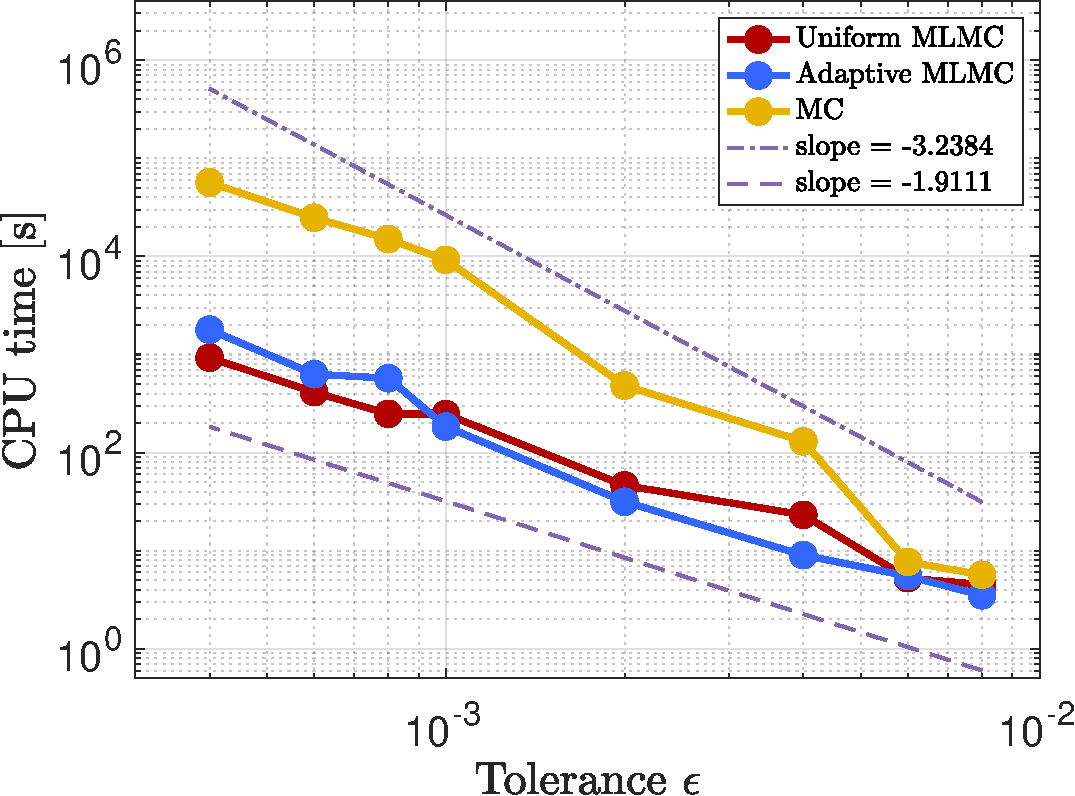
\includegraphics[height=0.35\linewidth]{CPUtime_epsilon_L2norm.pdf}&
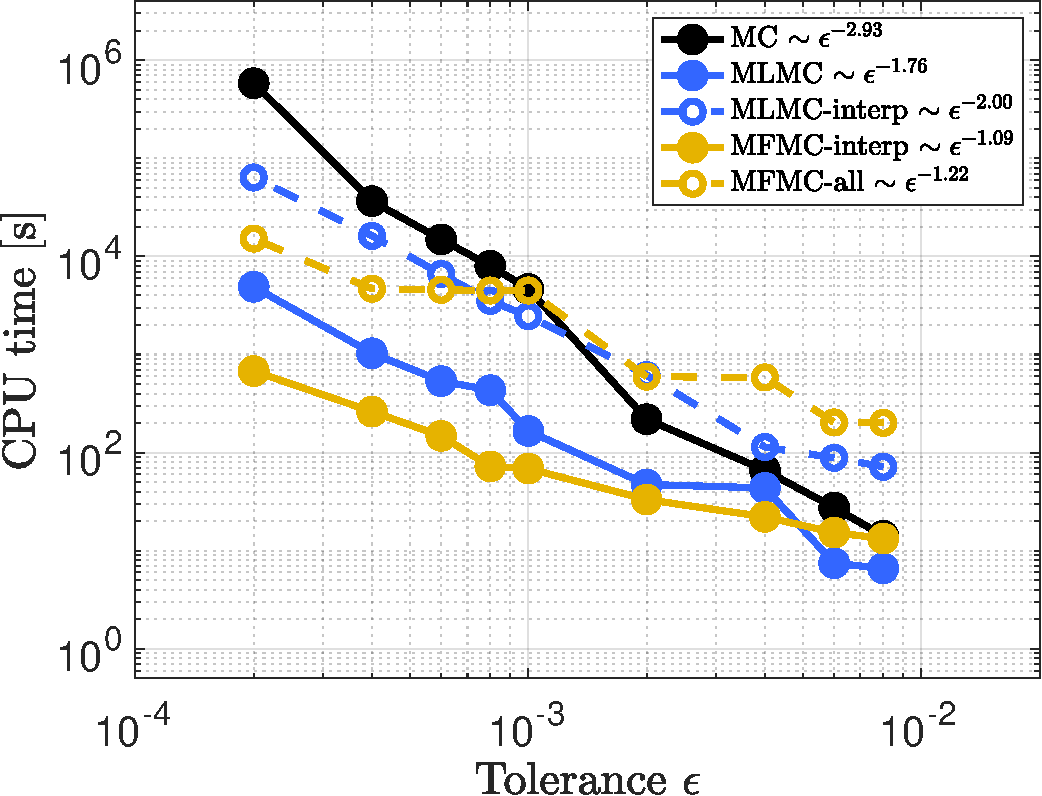
\includegraphics[height=0.4\linewidth]{Cost_epsilon.pdf}
\end{tabular}
}
% \caption{Left: sampling cost (CPU time in seconds) of direct computation vs. tolerance $\epsilon$ for MC, MLMC with geometry-conforming uniform meshes, and MLMC with adaptive meshes.  Right: sampling cost vs. tolerance $\epsilon$ for MC with both direct computation and surrogate, MLMC with both direct computation and surrogate.} 
\label{fig:Experiment_result_plot}
\end{figure}

\end{itemize}
\end{frame}

%------------------------------------------------------------
\begin{frame}[t]
    \frametitle{Approach 4: Multi-fidelity Monte Carlo}
\begin{itemize}[leftmargin=5pt] 
% \item[$\triangleright$] \textcolor{myblue3}{\bf Surrogate-enhanced multilevel Monte Carlo:} {\footnotesize Integrate surrogate with multilevel Monte Carlo.}
\item[$\triangleright$] \textcolor{myblue3}{\bf Accuracy:} 
{\footnotesize Plasma boundary and geometric descriptors from MFMC sampling exhibit behavior consistent with those from MC and MLMC when interpolated onto a common mesh.}
% \item[$\triangleright$] \textcolor{myblue3}{\bf Efficiency:} {\footnotesize 
%  Su.}
%  \vspace{3mm}
\begin{figure}[ht!]\centering
\scalebox{0.15}{
\begin{tabular}{cccc}
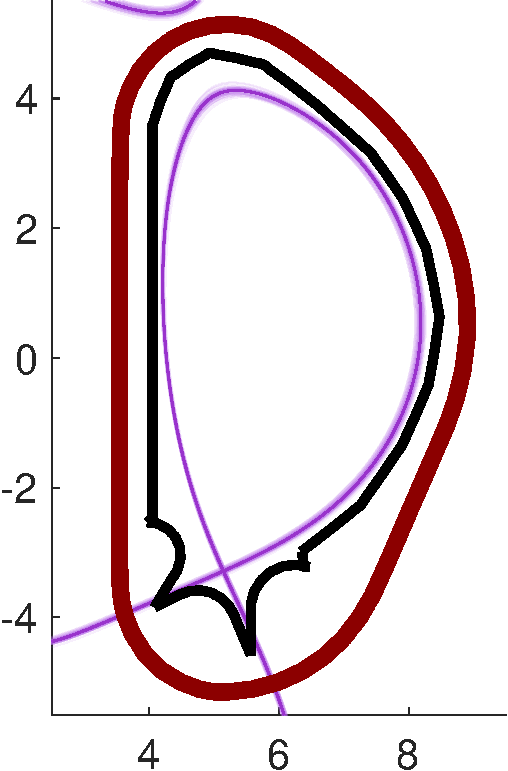
\includegraphics[width=1\linewidth]{QoI_MC_uniform.pdf}
&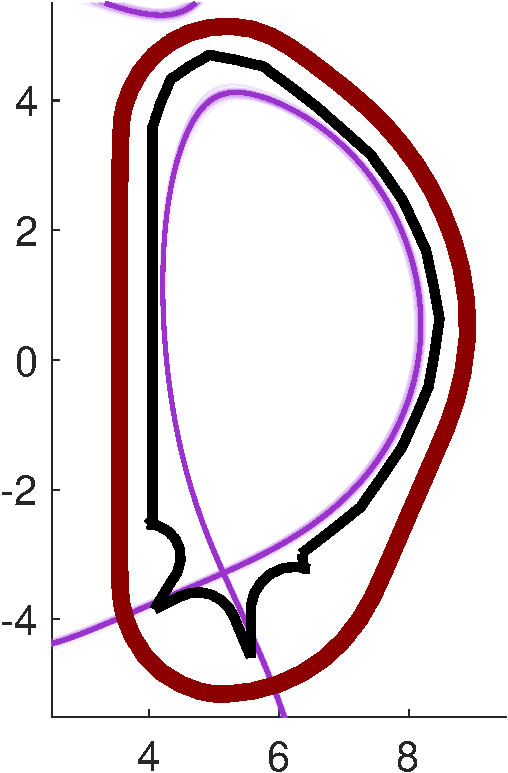
\includegraphics[width=1\linewidth]{QoI_MLMC_DirectSolver_Interp2CommonGrid.pdf}
&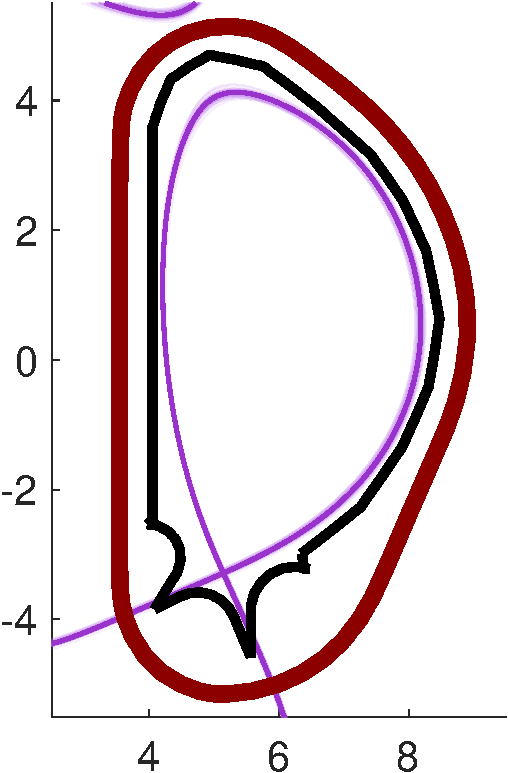
\includegraphics[width=1\linewidth]{QoI_MFMC.pdf} 
% &\includegraphics[width=1\linewidth]{QoI_MLMC_surrogate.pdf} 
% &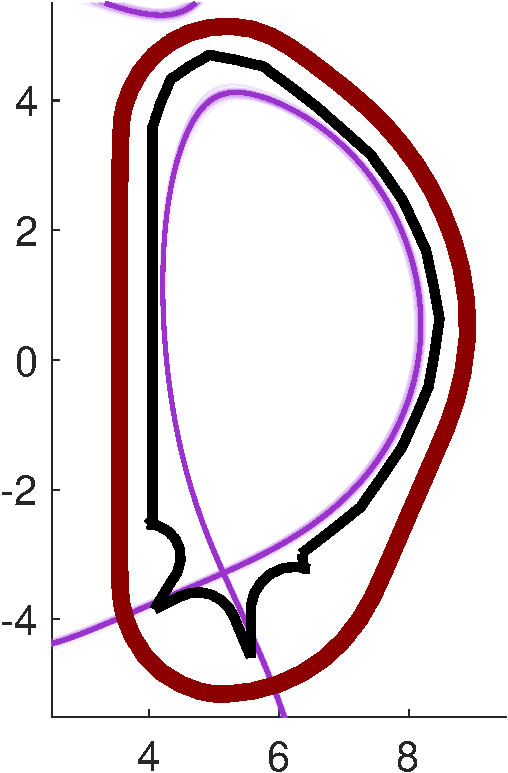
\includegraphics[width=1\linewidth]{QoI_MLMC_DirectSolver_Interp2CommonGrid.pdf} 
% &\includegraphics[width=1\linewidth]{QoI_MLMC_surrogate_Interp2CommonGrid.pdf} 
\\
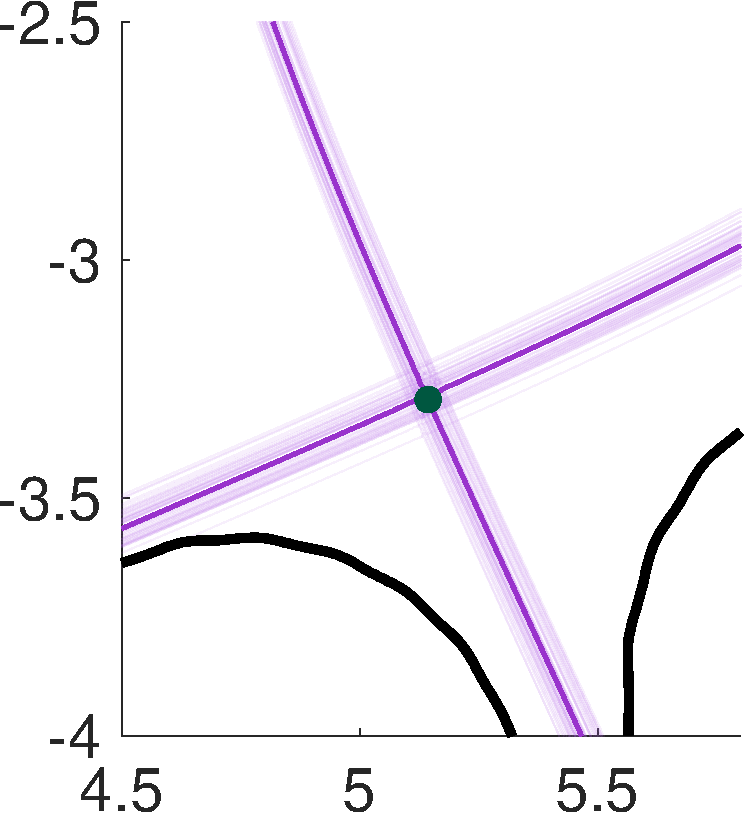
\includegraphics[width=1\linewidth]{QoI_MC_uniform_xptRegion.pdf} 
&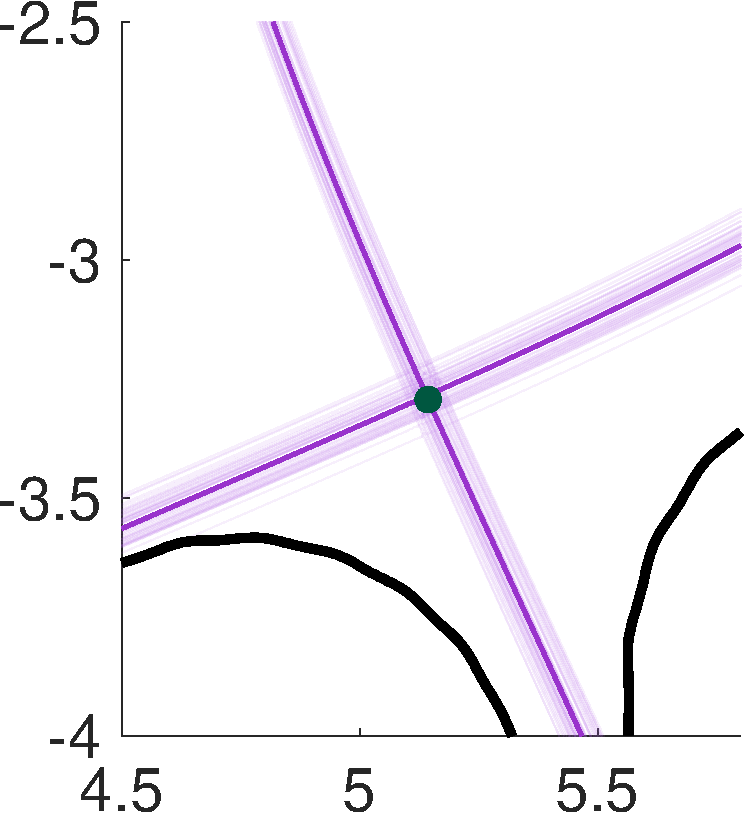
\includegraphics[width=1\linewidth]{QoI_MLMC_DirectSolver_xptRegion_Interp2CommonGrid.pdf} 
&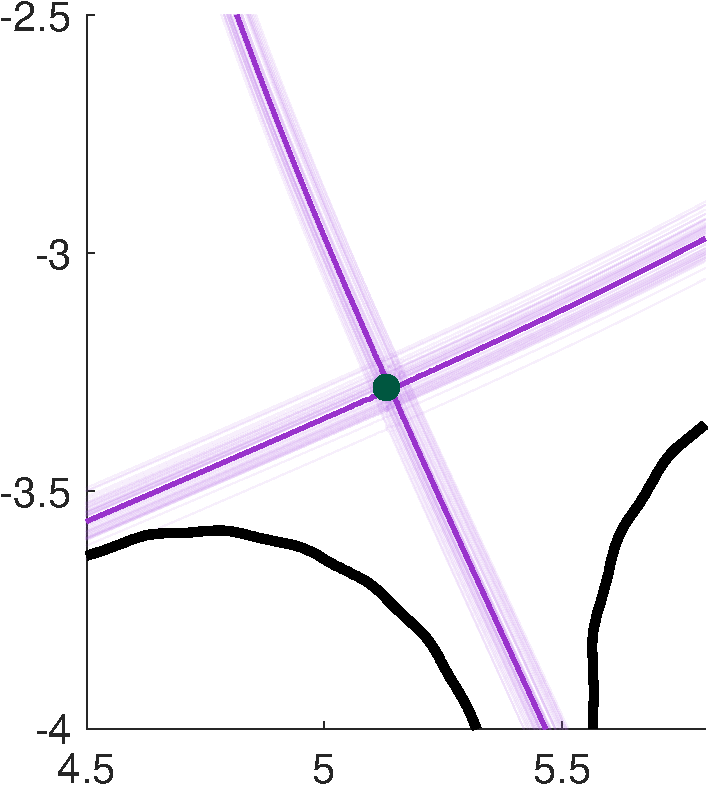
\includegraphics[width=1\linewidth]{QoI_MFMC_xptRegion.pdf} 
% &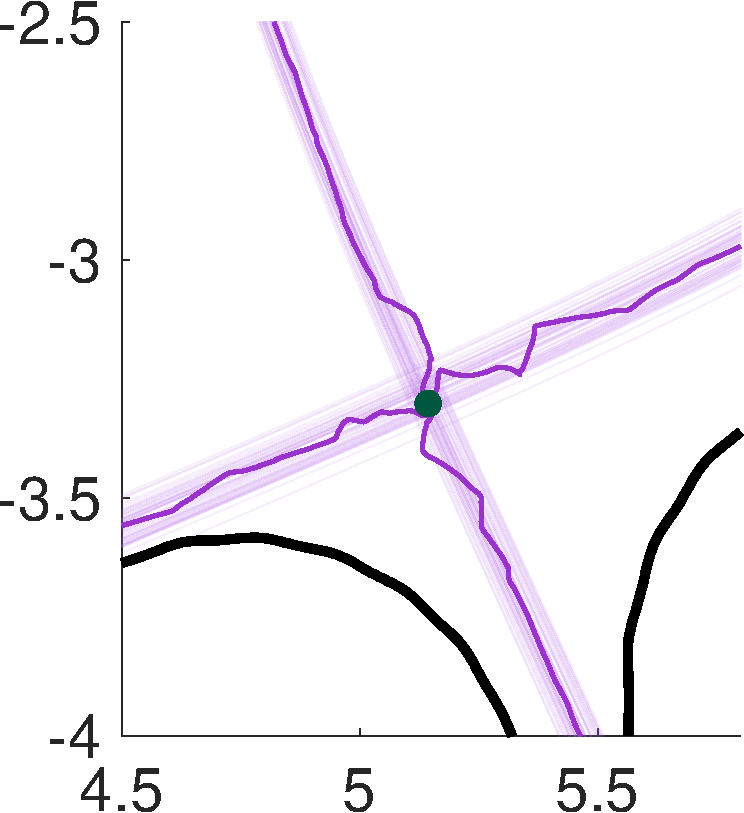
\includegraphics[width=1\linewidth]{QoI_MLMC_surrogate_xptRegion.pdf} 
% &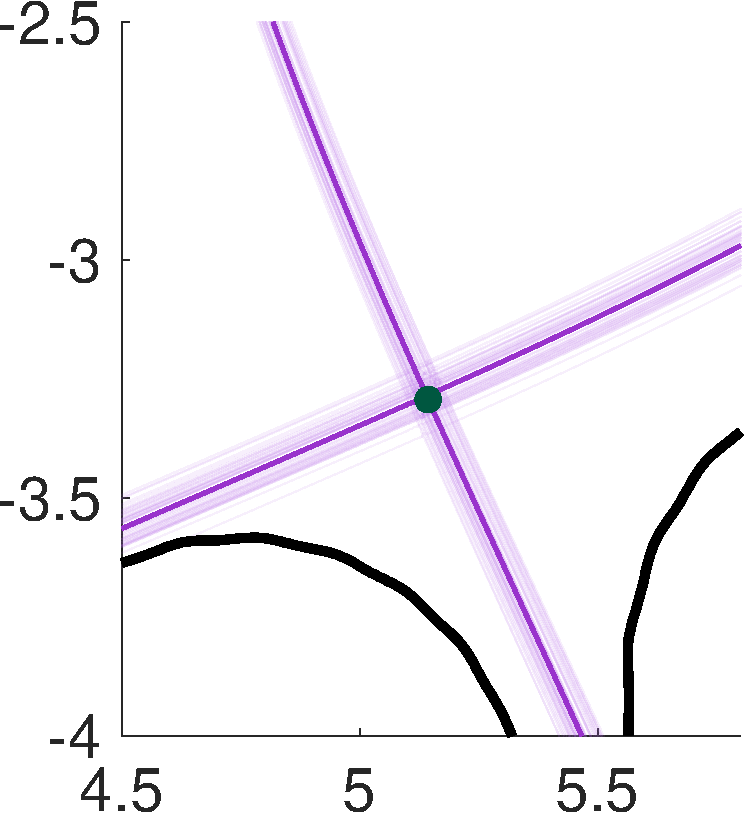
\includegraphics[width=1\linewidth]{QoI_MLMC_DirectSolver_xptRegion_Interp2CommonGrid.pdf}
% &\includegraphics[width=1\linewidth]{QoI_MLMC_surrogate_xptRegion_Interp2CommonGrid.pdf}
\\[1ex]
\quad {\fontsize{35}{35}\selectfont MC-FE} & {\fontsize{35}{35}\selectfont MLMC-FE (Interp)}  &{\fontsize{35}{35}\selectfont MFMC-FE (Interp)}
% & {\fontsize{35}{35}\selectfont MLMC + Direct + interp} 
% &{\fontsize{35}{35}\selectfont MLMC + Surrogate + interp} 
\\[-0.5ex]
\end{tabular}
}
\end{figure}


%
\vspace{1mm}
\item[$\triangleright$] {\bf This project is in preparation.}
\vspace{1mm}
        
% {\fontsize{8}{8}\selectfont \textcolor{mygray2}{In preparation.}
% \par}
\end{itemize}
\end{frame}

%-----------------------------------------------------------
\begin{frame}
% \frametitle{$|\!\!\sim\! \underline{\hspace{0.25cm}}\!\sim\!\! |@ \underline{\hspace{0.25cm}} @|\!* \!\underline{\hspace{0.25cm}}\!*\!|. \underline{\hspace{0.25cm}} .|- \underline{\hspace{0.25cm}} -|G \underline{\hspace{0.25cm}} G|x\underline{\hspace{0.25cm}} x|/\underline{\hspace{0.25cm}}\backslash|w_w|Q\underline{\hspace{0.25cm}}Q|>\underline{\hspace{0.25cm}}>|=\underline{\hspace{0.25cm}}=|+\underline{\hspace{0.25cm}}+|\#\underline{\hspace{0.25cm}}\#|z\underline{\hspace{0.25cm}}z|>\underline{\hspace{0.25cm}}<|6\underline{\hspace{0.25cm}}9|$}


	\begin{center}
	{\fontsize{35}{70}\selectfont  Thank You $|\neg\underline{\hspace{0.4cm}}\neg|$}
	\end{center}
\end{frame}
%----------------------------------------------------------------
\end{document}